% Generated by Sphinx.
\documentclass[a4paper,10pt,english]{manual}
\usepackage[utf8]{inputenc}
\usepackage[T1]{fontenc}
\usepackage{babel}
\usepackage{times}
\usepackage[Bjarne]{fncychap}
\usepackage{longtable}
\usepackage{sphinx}


\title{Workshop - FOSS4G routing with pgRouting tools, OpenStreetMap road data and GeoExt Manual}
\date{July 05, 2010}
\release{1}
\author{Daniel Kastl, Frédéric Junod}
\newcommand{\sphinxlogo}{}
\renewcommand{\releasename}{Release}
\makeindex


\makeatletter
\def\PYG@reset{\let\PYG@it=\relax \let\PYG@bf=\relax%
    \let\PYG@ul=\relax \let\PYG@tc=\relax%
    \let\PYG@bc=\relax \let\PYG@ff=\relax}
\def\PYG@tok#1{\csname PYG@tok@#1\endcsname}
\def\PYG@toks#1+{\ifx\relax#1\empty\else%
    \PYG@tok{#1}\expandafter\PYG@toks\fi}
\def\PYG@do#1{\PYG@bc{\PYG@tc{\PYG@ul{%
    \PYG@it{\PYG@bf{\PYG@ff{#1}}}}}}}
\def\PYG#1#2{\PYG@reset\PYG@toks#1+\relax+\PYG@do{#2}}

\def\PYG@tok@gd{\def\PYG@tc##1{\textcolor[rgb]{0.63,0.00,0.00}{##1}}}
\def\PYG@tok@gu{\let\PYG@bf=\textbf\def\PYG@tc##1{\textcolor[rgb]{0.50,0.00,0.50}{##1}}}
\def\PYG@tok@gt{\def\PYG@tc##1{\textcolor[rgb]{0.00,0.25,0.82}{##1}}}
\def\PYG@tok@gs{\let\PYG@bf=\textbf}
\def\PYG@tok@gr{\def\PYG@tc##1{\textcolor[rgb]{1.00,0.00,0.00}{##1}}}
\def\PYG@tok@cm{\let\PYG@it=\textit\def\PYG@tc##1{\textcolor[rgb]{0.25,0.50,0.56}{##1}}}
\def\PYG@tok@vg{\def\PYG@tc##1{\textcolor[rgb]{0.73,0.38,0.84}{##1}}}
\def\PYG@tok@m{\def\PYG@tc##1{\textcolor[rgb]{0.13,0.50,0.31}{##1}}}
\def\PYG@tok@mh{\def\PYG@tc##1{\textcolor[rgb]{0.13,0.50,0.31}{##1}}}
\def\PYG@tok@cs{\def\PYG@tc##1{\textcolor[rgb]{0.25,0.50,0.56}{##1}}\def\PYG@bc##1{\colorbox[rgb]{1.00,0.94,0.94}{##1}}}
\def\PYG@tok@ge{\let\PYG@it=\textit}
\def\PYG@tok@vc{\def\PYG@tc##1{\textcolor[rgb]{0.73,0.38,0.84}{##1}}}
\def\PYG@tok@il{\def\PYG@tc##1{\textcolor[rgb]{0.13,0.50,0.31}{##1}}}
\def\PYG@tok@go{\def\PYG@tc##1{\textcolor[rgb]{0.19,0.19,0.19}{##1}}}
\def\PYG@tok@cp{\def\PYG@tc##1{\textcolor[rgb]{0.00,0.44,0.13}{##1}}}
\def\PYG@tok@gi{\def\PYG@tc##1{\textcolor[rgb]{0.00,0.63,0.00}{##1}}}
\def\PYG@tok@gh{\let\PYG@bf=\textbf\def\PYG@tc##1{\textcolor[rgb]{0.00,0.00,0.50}{##1}}}
\def\PYG@tok@ni{\let\PYG@bf=\textbf\def\PYG@tc##1{\textcolor[rgb]{0.84,0.33,0.22}{##1}}}
\def\PYG@tok@nl{\let\PYG@bf=\textbf\def\PYG@tc##1{\textcolor[rgb]{0.00,0.13,0.44}{##1}}}
\def\PYG@tok@nn{\let\PYG@bf=\textbf\def\PYG@tc##1{\textcolor[rgb]{0.05,0.52,0.71}{##1}}}
\def\PYG@tok@no{\def\PYG@tc##1{\textcolor[rgb]{0.38,0.68,0.84}{##1}}}
\def\PYG@tok@na{\def\PYG@tc##1{\textcolor[rgb]{0.25,0.44,0.63}{##1}}}
\def\PYG@tok@nb{\def\PYG@tc##1{\textcolor[rgb]{0.00,0.44,0.13}{##1}}}
\def\PYG@tok@nc{\let\PYG@bf=\textbf\def\PYG@tc##1{\textcolor[rgb]{0.05,0.52,0.71}{##1}}}
\def\PYG@tok@nd{\let\PYG@bf=\textbf\def\PYG@tc##1{\textcolor[rgb]{0.33,0.33,0.33}{##1}}}
\def\PYG@tok@ne{\def\PYG@tc##1{\textcolor[rgb]{0.00,0.44,0.13}{##1}}}
\def\PYG@tok@nf{\def\PYG@tc##1{\textcolor[rgb]{0.02,0.16,0.49}{##1}}}
\def\PYG@tok@si{\let\PYG@it=\textit\def\PYG@tc##1{\textcolor[rgb]{0.44,0.63,0.82}{##1}}}
\def\PYG@tok@s2{\def\PYG@tc##1{\textcolor[rgb]{0.25,0.44,0.63}{##1}}}
\def\PYG@tok@vi{\def\PYG@tc##1{\textcolor[rgb]{0.73,0.38,0.84}{##1}}}
\def\PYG@tok@nt{\let\PYG@bf=\textbf\def\PYG@tc##1{\textcolor[rgb]{0.02,0.16,0.45}{##1}}}
\def\PYG@tok@nv{\def\PYG@tc##1{\textcolor[rgb]{0.73,0.38,0.84}{##1}}}
\def\PYG@tok@s1{\def\PYG@tc##1{\textcolor[rgb]{0.25,0.44,0.63}{##1}}}
\def\PYG@tok@gp{\let\PYG@bf=\textbf\def\PYG@tc##1{\textcolor[rgb]{0.78,0.36,0.04}{##1}}}
\def\PYG@tok@sh{\def\PYG@tc##1{\textcolor[rgb]{0.25,0.44,0.63}{##1}}}
\def\PYG@tok@ow{\let\PYG@bf=\textbf\def\PYG@tc##1{\textcolor[rgb]{0.00,0.44,0.13}{##1}}}
\def\PYG@tok@sx{\def\PYG@tc##1{\textcolor[rgb]{0.78,0.36,0.04}{##1}}}
\def\PYG@tok@bp{\def\PYG@tc##1{\textcolor[rgb]{0.00,0.44,0.13}{##1}}}
\def\PYG@tok@c1{\let\PYG@it=\textit\def\PYG@tc##1{\textcolor[rgb]{0.25,0.50,0.56}{##1}}}
\def\PYG@tok@kc{\let\PYG@bf=\textbf\def\PYG@tc##1{\textcolor[rgb]{0.00,0.44,0.13}{##1}}}
\def\PYG@tok@c{\let\PYG@it=\textit\def\PYG@tc##1{\textcolor[rgb]{0.25,0.50,0.56}{##1}}}
\def\PYG@tok@mf{\def\PYG@tc##1{\textcolor[rgb]{0.13,0.50,0.31}{##1}}}
\def\PYG@tok@err{\def\PYG@bc##1{\fcolorbox[rgb]{1.00,0.00,0.00}{1,1,1}{##1}}}
\def\PYG@tok@kd{\let\PYG@bf=\textbf\def\PYG@tc##1{\textcolor[rgb]{0.00,0.44,0.13}{##1}}}
\def\PYG@tok@ss{\def\PYG@tc##1{\textcolor[rgb]{0.32,0.47,0.09}{##1}}}
\def\PYG@tok@sr{\def\PYG@tc##1{\textcolor[rgb]{0.14,0.33,0.53}{##1}}}
\def\PYG@tok@mo{\def\PYG@tc##1{\textcolor[rgb]{0.13,0.50,0.31}{##1}}}
\def\PYG@tok@mi{\def\PYG@tc##1{\textcolor[rgb]{0.13,0.50,0.31}{##1}}}
\def\PYG@tok@kn{\let\PYG@bf=\textbf\def\PYG@tc##1{\textcolor[rgb]{0.00,0.44,0.13}{##1}}}
\def\PYG@tok@o{\def\PYG@tc##1{\textcolor[rgb]{0.40,0.40,0.40}{##1}}}
\def\PYG@tok@kr{\let\PYG@bf=\textbf\def\PYG@tc##1{\textcolor[rgb]{0.00,0.44,0.13}{##1}}}
\def\PYG@tok@s{\def\PYG@tc##1{\textcolor[rgb]{0.25,0.44,0.63}{##1}}}
\def\PYG@tok@kp{\def\PYG@tc##1{\textcolor[rgb]{0.00,0.44,0.13}{##1}}}
\def\PYG@tok@w{\def\PYG@tc##1{\textcolor[rgb]{0.73,0.73,0.73}{##1}}}
\def\PYG@tok@kt{\def\PYG@tc##1{\textcolor[rgb]{0.56,0.13,0.00}{##1}}}
\def\PYG@tok@sc{\def\PYG@tc##1{\textcolor[rgb]{0.25,0.44,0.63}{##1}}}
\def\PYG@tok@sb{\def\PYG@tc##1{\textcolor[rgb]{0.25,0.44,0.63}{##1}}}
\def\PYG@tok@k{\let\PYG@bf=\textbf\def\PYG@tc##1{\textcolor[rgb]{0.00,0.44,0.13}{##1}}}
\def\PYG@tok@se{\let\PYG@bf=\textbf\def\PYG@tc##1{\textcolor[rgb]{0.25,0.44,0.63}{##1}}}
\def\PYG@tok@sd{\let\PYG@it=\textit\def\PYG@tc##1{\textcolor[rgb]{0.25,0.44,0.63}{##1}}}

\def\PYGZbs{\char`\\}
\def\PYGZus{\char`\_}
\def\PYGZob{\char`\{}
\def\PYGZcb{\char`\}}
\def\PYGZca{\char`\^}
% for compatibility with earlier versions
\def\PYGZat{@}
\def\PYGZlb{[}
\def\PYGZrb{]}
\makeatother

\begin{document}

\maketitle
\tableofcontents
\hypertarget{--doc-latex}{}


\resetcurrentobjects
\hypertarget{--doc-chapters/introduction}{}

\chapter{Introduction}
\paragraph{Abstract}

\href{http://www.pgrouting.org}{pgRouting} adds routing functionality to \href{http://www.postgis.org}{PostGIS}. This introductory workshop will show you how. It gives a practical example of how to use pgRouting with \href{http://www.openstreetmap.org}{OpenStreetMap} road network data. It explains the steps to prepare the data, make routing queries, assign costs and use \href{http://www.geoext.org}{GeoExt} to show your route in a web-mapping application.

Navigation for road networks requires complex routing algorithms that support turn restrictions and even time-dependent attributes. pgRouting is an extendible open-source library that provides a variety of tools for shortest path search as extension of PostgreSQL and PostGIS. The workshop will explain about shortest path search with pgRouting in real road networks and how the data structure is important to get faster results. Also you will learn about difficulties and limitations of pgRouting in GIS applications.

To give a practical example the workshop makes use of OpenStreetMap data of Barcelona. You will learn how to convert the data into the required format and how to calibrate the data with ``cost'' attributes. Furthermore we will explain the difference of the main routing algorithms ``Dijkstra'', ``A-Star'' and ``Shooting-Star''. By the end of the workshop you will have a good understanding of how to use pgRouting and how to get your network data prepared.

To learn how to get the output from rows and columns to be drawn on a map, we will build a basic map GUI with GeoExt. We listened to the students feedback of the last year's and want to guide you through the basic steps to build a simple browser application. Our goal is to make this as easy as possible, and to show that it's not difficult to integrate with other FOSS4G tools. For that reason we selected GeoExt, which is a JavaScript library providing the groundwork for creating web-mapping applications based on OpenLayers and Ext.

\begin{notice}{note}{Note:}\begin{itemize}
\item {} 
Workshop level: intermediate

\item {} 
Attendee's previous knowledge: SQL (PostgreSQL, PostGIS), Javascript, HTML

\item {} 
Equipments: This workshops will make use of the GIS LiveDVD if possible. Otherwise it will require VirtualBox installed to load a virtual machine image.

\end{itemize}
\end{notice}
\paragraph{Presenter}
\begin{itemize}
\item {} 
\emph{Daniel Kastl} is founder and CEO of \href{http://georepublic.de}{Georepublic UG} and works in Germany and Japan. He is moderating and promoting the pgRouting community and development since 4 years, and he's an active OSM contributor in Japan.

\item {} 
\emph{Frédéric Junod} works at the Swiss office of \href{http://www.camptocamp.com}{Camptocamp} for about five years. He's an active developer of many open source GIS projects from the browser (GeoExt, OpenLayers) to the server world (MapFish, Shapely, TileCache) and he is member of the pgRouting PSC.

\end{itemize}

Daniel and Frédéric are the auhtors of the previous pgRouting workshops, that have been held at FOSS4G events in Canada and South Africa and at local conferences in Japan.
\paragraph{License}

This work is licensed under a \href{http://creativecommons.org/licenses/by-sa/3.0/}{Creative Commons Attribution-Share Alike 3.0 License}.


\includegraphics{license.png}
\paragraph{Supported by}


\includegraphics{camptocamp.png}

\href{http://www.camptocamp.com}{Camptocamp}


\includegraphics{georepublic.png}

\href{http://georepublic.de}{Georepublic}

\resetcurrentobjects
\hypertarget{--doc-chapters/about}{}

\chapter{About}

This workshop makes use of several FOSS4G tools, a lot more than the workshop title mentions. Also a lot of FOSS4G software is related to other open source projects and it would go too far to list them all. These are the four FOSS4G projects this workshop will focus on:


\includegraphics{osgeo.png}


\section{pgRouting}

pgRouting is an extension of PostGIS and adds routing functionality to PostGIS/PostgreSQL. pgRouting is a further development of pgDijkstra (by \href{http://www.camptocamp.com}{Camptocamp SA}). It was extended by \href{http://www.orkney.co.jp}{Orkney Inc.}, and is currently developed and maintained by \href{http://georepublic.de}{Georepublic}.


\includegraphics{pgrouting.png}

pgRouting provides functions for:
\begin{itemize}
\item {} 
Shortest Path Dikstra: routing algorithm without heuristics

\item {} 
Shortest Path A-Star: routing for large datasets (with heuristics)

\item {} 
Shortest Path Shooting-Star: routing with turn restrictions (with heuristics)

\item {} 
Traveling Salesperson Problem (TSP)

\item {} 
Driving Distance calculation (Isolines)

\end{itemize}

Advantages of the database routing approach are:
\begin{itemize}
\item {} 
Accessible by multiple clients through JDBC, ODBC, or directly using Pl/pgSQL. The clients can either be PCs or mobile devices.

\item {} 
Uses PostGIS for its geographic data format, which in turn uses OGC's data format Well Konwn Text (WKT) and Well Known Binary (WKB). This allows usage of existing open * data converters.

\item {} 
Open Source software like qGIS and uDig can modify the data/attributes,

\item {} 
Data changes can be reflected instantaneously through the routing engine. There is no need for precalculation.

\item {} 
The ``cost'' parameter can be dynamically calculated through SQL and its value can come from multiple fields or tables.

\end{itemize}

pgRouting is available under the GPLv2 license.

pgRouting website: \href{http://www.pgrouting.org}{http://www.pgrouting.org}


\section{OpenStreetMap}

\emph{``OpenStreetMap is a project aimed squarely at creating and providing free geographic data such as street maps to anyone who wants them. The project was started because most maps you think of as free actually have legal or technical restrictions on their use, holding back people from using them in creative, productive or unexpected ways.''} (Source: \href{http://wiki.openstreetmap.org/index.php/Press}{http://wiki.openstreetmap.org/index.php/Press})

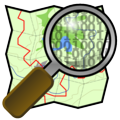
\includegraphics{osm_logo.png}

OpenStreetMap is a perfect data source to use for pgRouting, because it's freely available and has no technical restrictions in terms of processing the data. Data availability still varies from country to country, but the worldwide coverage is improving day by day.

OpenStreetMap uses a topological data structure:
\begin{itemize}
\item {} 
Nodes are points with a geographic position.

\item {} 
Ways are lists of nodes, representing a polyline or polygon.

\item {} 
Relations are groups of nodes, ways and other relations which can be assigned certain properties.

\item {} 
Tags can be applied to nodes, ways or relations and consist of name=value pairs.

\end{itemize}

OpenStreetMap website: \href{http://www.openstreetmap.org}{http://www.openstreetmap.org}


\section{osm2pgrouting}

osm2pgrouting is a command line tool that makes it easy to import OpenStreetMap data into a pgRouting database. It builds the routing network topology automatically and creates tables for feature types and road classes. osm2pgrouting was primarily written by Daniel Wendt and is now hosted on the pgRouting project site.

osm2pgrouting is available under the GPLv2 license.

Project website: \href{http://pgrouting.postlbs.org/wiki/tools/osm2pgrouting}{http://pgrouting.postlbs.org/wiki/tools/osm2pgrouting}


\section{GeoExt}

GeoExt is a ``JavaScript Toolkit for Rich Web Mapping Applications''. GeoExt brings together the geospatial know how of \href{http://www.openlayers.org}{OpenLayers} with the user interface savvy of \href{http://www.sencha.com}{Ext JS} to help you build powerful desktop style GIS apps on the web with JavaScript.


\includegraphics{GeoExt.png}

GeoExt is available under the BSD license and is supported by a growing community of individuals, businesses and organizations.

GeoExt website: \href{http://www.geoext.org}{http://www.geoext.org}

\resetcurrentobjects
\hypertarget{--doc-chapters/installation}{}

\chapter{Installation and Requirements}

For this workshop you need:
\begin{itemize}
\item {} 
A webserver like Apache with PHP support (and PHP PostgreSQL module)

\item {} 
Preferrable a Linux operating system like Ubuntu

\item {} 
An editor like Gedit

\item {} 
Internet connection

\end{itemize}

All required tools are available on the OSGeo LiveDVD, so the following reference is a quick summary of how to install it on your own computer running latest Ubuntu 10.04.


\section{Software}

Installation of pgRouting on Ubuntu became very easy now because packages are available in a \href{https://launchpad.net/~georepublic/+archive/pgrouting}{Launchpad repository}:

All you need to do now is to open a terminal window and run:

\begin{Verbatim}[commandchars=\\\{\}]
\PYG{c}{\# Add pgRouting launchpad repository}
sudo add-apt-repository ppa:georepublic/pgrouting
sudo apt-get update

\PYG{c}{\# Install pgRouting packages}
sudo apt-get install gaul-devel \PYG{l+s+se}{\PYGZbs{}}
        postgresql-8.4-pgrouting \PYG{l+s+se}{\PYGZbs{}}
        postgresql-8.4-pgrouting-dd \PYG{l+s+se}{\PYGZbs{}}
        postgresql-8.4-pgrouting-tsp

\PYG{c}{\# Install osm2pgrouting package}
sudo apt-get install osm2pgrouting

\PYG{c}{\# Install workshop material (optional)}
sudo apt-get install pgrouting-workshop
\end{Verbatim}

This will also install all required packages such as PostgreSQL and PostGIS if not installed yet.

\begin{notice}{note}{Note:}\begin{itemize}
\item {} 
``Multiverse'' packages must be available as software sources. Currently only packages for Ubuntu 10.04 have been built, but further packages are likely to come if there is demand for them.

\item {} 
To be up-to-date with changes and improvements you might run \code{sudo apt-get update \& sudo apt-get upgrade} from time to time, especially if you use an older version of the LiveDVD.

\item {} 
To avoid permission denied errors for local users you can set connection method to \code{trust} in \code{/etc/postgresql/8.4/main/pg\_hba.conf} and restart PostgreSQL server with \code{sudo service postgresql-8.4 restart}.

\end{itemize}
\end{notice}


\section{Data}

The pgRouting workshop will make use of OpenStreetMap data of Barcelona, which is already available on the LiveDVD. If you don't use the LiveDVD or want to download the latest data or the data of your choice, you can make use of OpenStreetMap's API from your terminal window:

\begin{Verbatim}[commandchars=\\\{\}]
\PYG{c}{\# Dowload as file barcelona.osm}
wget --progress\PYG{o}{=}dot:mega -O barcelona.osm \PYG{l+s+se}{\PYGZbs{}}
        http://osmxapi.hypercube.telascience.org/api/0.6/map?bbox\PYG{o}{=}1.998653,41.307213,2.343693,41.495207
\end{Verbatim}

The API has a download size limitation, which can make it a bit inconvenient to download large areas with many features. An alternative is \href{http://josm.openstreetmap.de}{JOSM Editor}, which also makes API calls to dowload data, but it provides an user friendly interface. You can save the data as \code{.osm} file to use it in this workship. JOSM is also available on the LiveDVD.

\begin{notice}{note}{Note:}\begin{itemize}
\item {} 
OpenStreetMap API v0.6, see for more information \href{http://wiki.openstreetmap.org/index.php/OSM\_Protocol\_Version\_0.6}{http://wiki.openstreetmap.org/index.php/OSM\_Protocol\_Version\_0.6} .

\item {} 
Barcelona data is available at the LiveDVD in \code{/usr/local/share/osm/}

\end{itemize}
\end{notice}

An alternative for very large areas is the download service of \href{http://www.cloudemade.com}{CloudMade}. The company offers extracts of maps from countries around the world. For data of Spain for example go to \href{http://download.cloudmade.com/europe/spain}{http://download.cloudmade.com/europe/spain} and download the compressed \code{.osm.bz2} file:

\begin{Verbatim}[commandchars=\\\{\}]
wget --progress\PYG{o}{=}dot:mega http://download.cloudmade.com/europe/spain/spain.osm.bz2
\end{Verbatim}

\begin{notice}{warning}{Warning:}
Data of a whole country might be too big for the LiveDVD as well as processing time might take very long.
\end{notice}


\section{Workshop}

If you installed the workshop package you will find all documents in \code{/usr/share/pgrouting/workshop/}.

We recommend to copy the files to your home directory and make a symbolic link to your webserver's root folder:

\begin{Verbatim}[commandchars=\\\{\}]
cp -R /usr/share/pgrouting/workshop \textasciitilde{}/Desktop/pgrouting-workshop
sudo ln -s \textasciitilde{}/Desktop/pgrouting-workshop/web /var/www/pgrouting-workshop
\end{Verbatim}

You can then find all workshop files in the \code{pgrouting-workshop} folder and access to
\begin{itemize}
\item {} 
Web directory: \href{http://localhost/pgrouting-workshop}{http://localhost/pgrouting-workshop}

\item {} 
Online manual: \href{http://localhost/pgrouting-workshop/docs/\_build/html/index.html}{http://localhost/pgrouting-workshop/docs/\_build/html/index.html}

\end{itemize}

\begin{notice}{note}{Note:}
Additional sample data is available in the workshop \code{data} directory. It contains a compressed file with database dumps as well as a smaller network data of Barcelona downtown. To extract the file run \code{tar -xzf \textasciitilde{}/Desktop/pgrouting-workshop/data/sampledata.tar.gz}.
\end{notice}

\resetcurrentobjects
\hypertarget{--doc-chapters/osm2pgrouting}{}

\chapter{osm2pgrouting Import Tool}

osm2pgrouting is a command line tool that makes it very easy to import OpenStreetMap data into a pgRouting database. It builds the routing network topology automatically and creates tables for feature types and road classes. osm2pgrouting was primarily written by Daniel Wendt and is currently hosted on the pgRouting project site: \href{http://pgrouting.postlbs.org/wiki/tools/osm2pgrouting}{http://pgrouting.postlbs.org/wiki/tools/osm2pgrouting}

\begin{notice}{note}{Note:}
There are some limitations though especially regarding network size. The current version of osm2pgrouting needs to load all data into memory, which makes it fast but also requires a lot or memory for large datasets. An alternative tool to osm2pgrouting without the network size limitation is \emph{osm2po}. It's available as under a ``freeware license'' (not open source license unfortunately)
\end{notice}

Raw OpenStreetMap data contains much more features and information than need for routing. Also the format is not suitable for pgRouting out-of-the-box. An \code{.osm} XML file consists of three major feature types:
\begin{itemize}
\item {} 
nodes

\item {} 
ways

\item {} 
relations

\end{itemize}

The data of Barcelona.osm for example looks like this:

\begin{Verbatim}[commandchars=@\[\]]
@textless[]?xml version='1.0' encoding='UTF-8'?@textgreater[]
@textless[]osm version='0.6' generator='xapi: OSM Extended API 2.0' ... @textgreater[]
  ...	
  @textless[]node id='255405560' lat='41.4917468' lon='2.0257695' version='1' 
  		changeset='19117' user='efrainlarrea' uid='32823' visible='true' 
  		timestamp='2008-04-02T17:40:07Z'@textgreater[]
  @textless[]/node@textgreater[]
  @textless[]node id='255405551' lat='41.4866740' lon='2.0302842' version='3' 
  		changeset='248452' user='efrainlarrea' uid='32823' visible='true' 
  		timestamp='2008-04-24T15:56:08Z'@textgreater[]
  @textless[]/node@textgreater[]
  @textless[]node id='255405552' lat='41.4868540' lon='2.0297863' version='1' 
  		changeset='19117' user='efrainlarrea' uid='32823' visible='true' 
  		timestamp='2008-04-02T17:40:07Z'@textgreater[]
  @textless[]/node@textgreater[]
  ...
  @textless[]way id='35419222' visible='true' timestamp='2009-06-03T21:49:11Z' 
  		version='1' changeset='1416898' user='Yodeima' uid='115931'@textgreater[]
    @textless[]nd ref='415466914'/@textgreater[]
    @textless[]nd ref='415466915'/@textgreater[]
    @textless[]tag k='highway' v='unclassified'/@textgreater[]
    @textless[]tag k='lanes' v='1'/@textgreater[]
    @textless[]tag k='name' v='Carrer del Progrés'/@textgreater[]
    @textless[]tag k='oneway' v='no'/@textgreater[]
  @textless[]/way@textgreater[]
  @textless[]way id='35419227' visible='true' timestamp='2009-06-14T20:37:55Z' 
  		version='2' changeset='1518775' user='Yodeima' uid='115931'@textgreater[]
    @textless[]nd ref='415472085'/@textgreater[]
    @textless[]nd ref='415472086'/@textgreater[]
    @textless[]nd ref='415472087'/@textgreater[]
    @textless[]tag k='highway' v='unclassified'/@textgreater[]
    @textless[]tag k='lanes' v='1'/@textgreater[]
    @textless[]tag k='name' v='carrer de la mecanica'/@textgreater[]
    @textless[]tag k='oneway' v='no'/@textgreater[]
  @textless[]/way@textgreater[]
  ...
  @textless[]relation id='903432' visible='true' timestamp='2010-05-06T08:36:54Z' 
  		version='1' changeset='4619553' user='ivansanchez' uid='5265'@textgreater[]
    @textless[]member type='way' ref='56426179' role='outer'/@textgreater[]
    @textless[]member type='way' ref='56426173' role='inner'/@textgreater[]
    @textless[]tag k='layer' v='0'/@textgreater[]
    @textless[]tag k='leisure' v='common'/@textgreater[]
    @textless[]tag k='name' v='Plaça Can Suris'/@textgreater[]
    @textless[]tag k='source' v='WMS shagrat.icc.cat'/@textgreater[]
    @textless[]tag k='type' v='multipolygon'/@textgreater[]
  @textless[]/relation@textgreater[]
  ...
@textless[]/osm@textgreater[]
\end{Verbatim}

Detailed description of all possible OpenStretMap types and classes can be found here:  \href{http://wiki.openstreetmap.org/index.php/Map\_features}{http://wiki.openstreetmap.org/index.php/Map\_features}.

When using osm2pgrouting, we take only nodes and ways of types and classes specified in \code{mapconfig.xml} file that will be imported into the routing database:

\begin{Verbatim}[commandchars=\\\{\}]
\PYG{c+cp}{\textless{}?xml version="1.0" encoding="UTF-8"?\textgreater{}}
\PYG{n+nt}{\textless{}configuration}\PYG{n+nt}{\textgreater{}}
  \PYG{n+nt}{\textless{}type} \PYG{n+na}{name=}\PYG{l+s}{"highway"} \PYG{n+na}{id=}\PYG{l+s}{"1"}\PYG{n+nt}{\textgreater{}}
    \PYG{n+nt}{\textless{}class} \PYG{n+na}{name=}\PYG{l+s}{"motorway"} \PYG{n+na}{id=}\PYG{l+s}{"101"} \PYG{n+nt}{/\textgreater{}}
    \PYG{n+nt}{\textless{}class} \PYG{n+na}{name=}\PYG{l+s}{"motorway\PYGZus{}link"} \PYG{n+na}{id=}\PYG{l+s}{"102"} \PYG{n+nt}{/\textgreater{}}
    \PYG{n+nt}{\textless{}class} \PYG{n+na}{name=}\PYG{l+s}{"motorway\PYGZus{}junction"} \PYG{n+na}{id=}\PYG{l+s}{"103"} \PYG{n+nt}{/\textgreater{}}
    ...
    \PYG{n+nt}{\textless{}class} \PYG{n+na}{name=}\PYG{l+s}{"road"} \PYG{n+na}{id=}\PYG{l+s}{"100"} \PYG{n+nt}{/\textgreater{}}
  \PYG{n+nt}{\textless{}/type\textgreater{}}    
  \PYG{n+nt}{\textless{}type} \PYG{n+na}{name=}\PYG{l+s}{"junction"} \PYG{n+na}{id=}\PYG{l+s}{"4"}\PYG{n+nt}{\textgreater{}}
    \PYG{n+nt}{\textless{}class} \PYG{n+na}{name=}\PYG{l+s}{"roundabout"} \PYG{n+na}{id=}\PYG{l+s}{"401"} \PYG{n+nt}{/\textgreater{}}
  \PYG{n+nt}{\textless{}/type\textgreater{}}  
\PYG{n+nt}{\textless{}/configuration\textgreater{}}
\end{Verbatim}

The default \code{mapconfig.xml} is installed in \code{/usr/share/osm2pgrouting/}.


\section{Create pgRouting database}

Before we can run osm2pgrouting we have to create PostgreSQL database and load PostGIS and pgRouting functions into this database. Therefor open a terminal window and execute the following commands:

\begin{Verbatim}[commandchars=\\\{\}]
\PYG{c}{\# become user "postgres" (or run as user "postgres")}
sudo su postgres

\PYG{c}{\# create routing database}
createdb routing
createlang plpgsql routing

\PYG{c}{\# add PostGIS functions}
psql -d routing -f /usr/share/postgresql/8.4/contrib/postgis-1.5/postgis.sql
psql -d routing -f /usr/share/postgresql/8.4/contrib/postgis-1.5/spatial\PYGZus{}ref\PYGZus{}sys.sql

\PYG{c}{\# add pgRouting core functions}
psql -d routing -f /usr/share/postlbs/routing\PYGZus{}core.sql
psql -d routing -f /usr/share/postlbs/routing\PYGZus{}core\PYGZus{}wrappers.sql
psql -d routing -f /usr/share/postlbs/routing\PYGZus{}topology.sql
\end{Verbatim}

An alternative way with PgAdmin III and SQL commands. Start PgAdmin III (available on the LiveDVD), connect to any database and open the SQL Editor:

\begin{Verbatim}[commandchars=\\\{\}]
\PYG{c+c1}{-- create routing database}
\PYG{k}{CREATE} \PYG{k}{DATABASE} \PYG{l+s+ss}{"routing"}\PYG{p}{;}
\end{Verbatim}

Then connect to the \code{routing} database and open a new SQL Editor window:

\begin{Verbatim}[commandchars=\\\{\}]
\PYG{c+c1}{-- add plpgsql and PostGIS/pgRouting functions}
\PYG{k}{CREATE} \PYG{k}{PROCEDURAL} \PYG{k}{LANGUAGE} \PYG{n}{plpgsql}\PYG{p}{;}
\end{Verbatim}

Next open \code{.sql} files with PostGIS/pgRouting functions as above and load them to the \code{routing} database.

\begin{notice}{note}{Note:}
PostGIS \code{.sql} files can be on different locations. This depends on your version of PostGIS and PostgreSQL. The example above is valid for PostgeSQL/PostGIS versions installed on the LiveDVD.
\end{notice}


\section{Run osm2pgrouting}

The next step is to run \code{osm2pgrouting} converter, which is a command line tool, so you need to open a terminal window.

We take the default \code{mapconfig.xml} configuration file and the \code{routing} database we created before. Furthermore we take \code{\textasciitilde{}/Desktop/pgrouting-workshop/data/sampledata.osm} as raw data. This file contains only OSM data from downtown Barcelona to speed up  data processing time.

\begin{Verbatim}[commandchars=\\\{\}]
osm2pgrouting   -file \PYG{l+s+s2}{"\textasciitilde{}/Desktop/pgrouting-workshop/data/sampledata.osm"} \PYG{l+s+se}{\PYGZbs{}}
                                -conf \PYG{l+s+s2}{"/usr/share/osm2pgrouting/mapconfig.xml"} \PYG{l+s+se}{\PYGZbs{}}
                                -dbname routing \PYG{l+s+se}{\PYGZbs{}}
                                -user postgres \PYG{l+s+se}{\PYGZbs{}}
                                -clean
\end{Verbatim}

A list of all possible parameters:
\begin{itemize}
\item {} 
required
\begin{itemize}
\item {} 
\code{file    \textless{}file\textgreater{}      -{-} name of your osm xml file}

\item {} 
\code{dbname  \textless{}dbname\textgreater{}    -{-} name of your database}

\item {} 
\code{user    \textless{}user\textgreater{}      -{-} name of the user, which have write access to the database}

\item {} 
\code{conf    \textless{}file\textgreater{}      -{-} name of your configuration xml file}

\end{itemize}

\item {} 
optional
\begin{itemize}
\item {} 
\code{host    \textless{}host\textgreater{}      -{-} host of your postgresql database (default: 127.0.0.1)}

\item {} 
\code{port    \textless{}port\textgreater{}      -{-} port of your database (default: 5432)}

\item {} 
\code{passwd  \textless{}passwd\textgreater{}    -{-}  password for database access}

\item {} 
\code{clean               -{-} drop peviously created tables}

\end{itemize}

\end{itemize}

\begin{notice}{note}{Note:}
If you get permission denied error for postgres users you can set connection method to \code{trust} in \code{/etc/postgresql/8.4/main/pg\_hba.conf} and restart PostgreSQL server with \code{sudo service postgresql-8.4 restart}.
\end{notice}

Depending on the size of your network the calculation and import may take a while. After it's finished connect to your database and check the tables that should have been created:
\paragraph{Run: \code{psql -U postgres -d routing -c "\textbackslash{}d"}}

\begin{Verbatim}[commandchars=\\\{\}]
                     \PYG{n}{List} \PYG{k}{of} \PYG{n}{relations}
 \PYG{k}{Schema} \PYG{o}{\textbar{}}        \PYG{n}{Name}         \PYG{o}{\textbar{}}   \PYG{k}{Type}   \PYG{o}{\textbar{}}  \PYG{k}{Owner}
\PYG{c+c1}{--------+---------------------+----------+----------}
 \PYG{k}{public} \PYG{o}{\textbar{}} \PYG{n}{classes}             \PYG{o}{\textbar{}} \PYG{k}{table}    \PYG{o}{\textbar{}} \PYG{n}{postgres}
 \PYG{k}{public} \PYG{o}{\textbar{}} \PYG{n}{geometry\PYGZus{}columns}    \PYG{o}{\textbar{}} \PYG{k}{table}    \PYG{o}{\textbar{}} \PYG{n}{postgres}
 \PYG{k}{public} \PYG{o}{\textbar{}} \PYG{n}{nodes}               \PYG{o}{\textbar{}} \PYG{k}{table}    \PYG{o}{\textbar{}} \PYG{n}{postgres}
 \PYG{k}{public} \PYG{o}{\textbar{}} \PYG{n}{spatial\PYGZus{}ref\PYGZus{}sys}     \PYG{o}{\textbar{}} \PYG{k}{table}    \PYG{o}{\textbar{}} \PYG{n}{postgres}
 \PYG{k}{public} \PYG{o}{\textbar{}} \PYG{n}{types}               \PYG{o}{\textbar{}} \PYG{k}{table}    \PYG{o}{\textbar{}} \PYG{n}{postgres}
 \PYG{k}{public} \PYG{o}{\textbar{}} \PYG{n}{vertices\PYGZus{}tmp}        \PYG{o}{\textbar{}} \PYG{k}{table}    \PYG{o}{\textbar{}} \PYG{n}{postgres}
 \PYG{k}{public} \PYG{o}{\textbar{}} \PYG{n}{vertices\PYGZus{}tmp\PYGZus{}id\PYGZus{}seq} \PYG{o}{\textbar{}} \PYG{n}{sequence} \PYG{o}{\textbar{}} \PYG{n}{postgres}
 \PYG{k}{public} \PYG{o}{\textbar{}} \PYG{n}{ways}                \PYG{o}{\textbar{}} \PYG{k}{table}    \PYG{o}{\textbar{}} \PYG{n}{postgres}
\PYG{p}{(}\PYG{l+m+mi}{8} \PYG{k}{rows}\PYG{p}{)}
\end{Verbatim}

If everything went well the result should look like this:

\resetcurrentobjects
\hypertarget{--doc-chapters/topology}{}

\chapter{Load road data and create a network topology}

{\hfill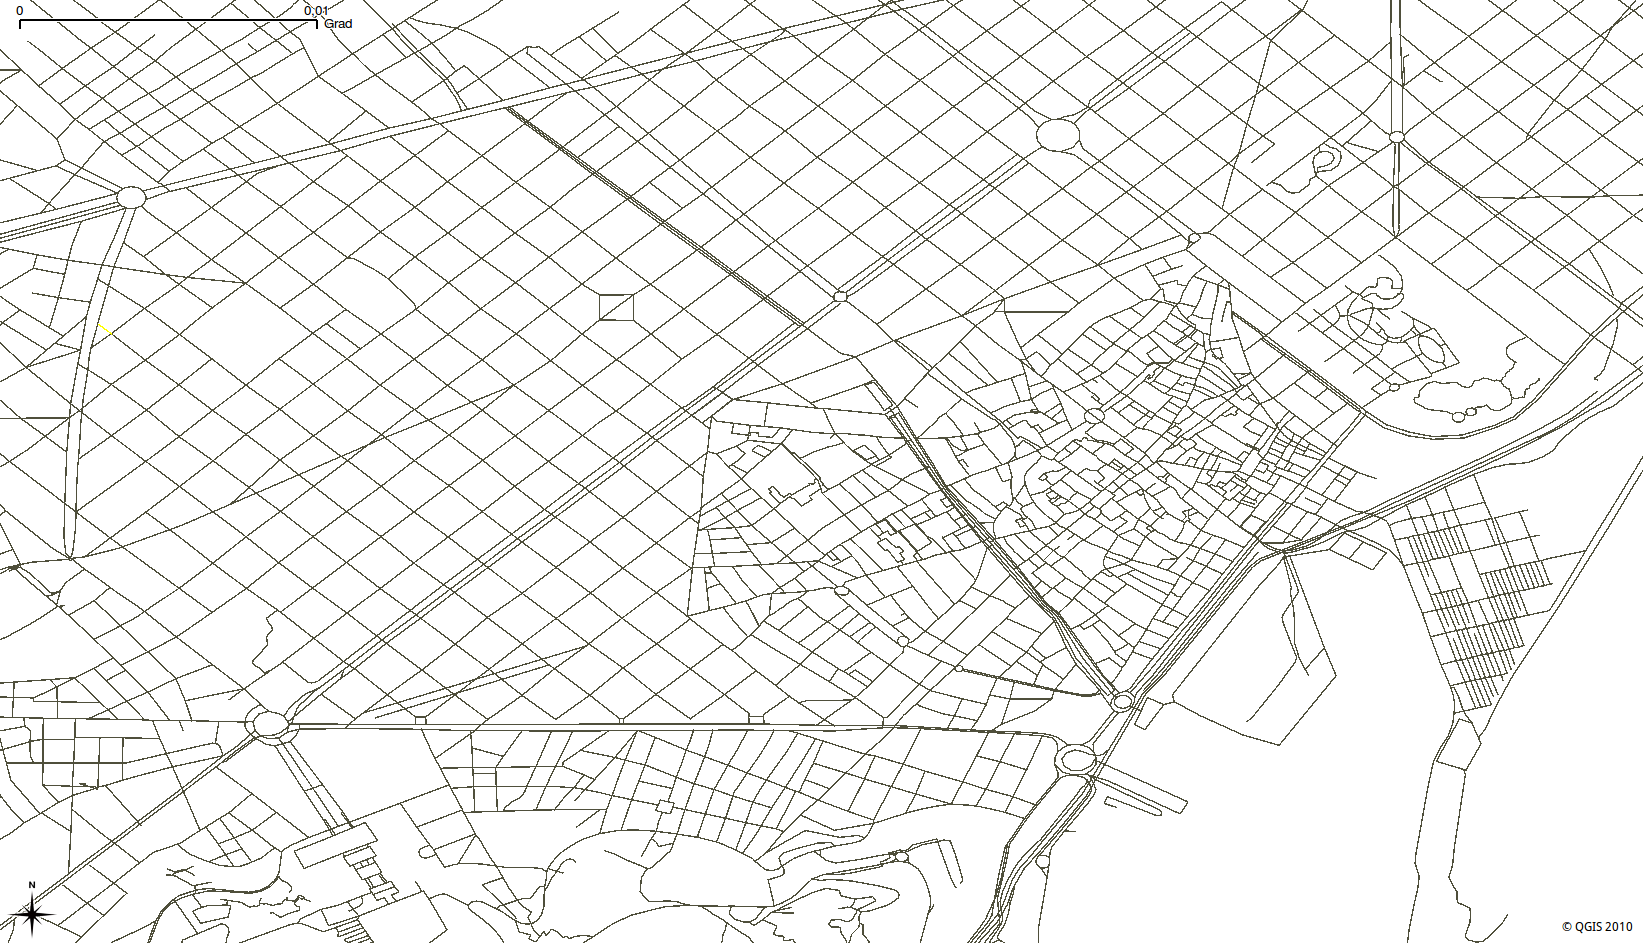
\includegraphics[width=250pt]{network.png}\hfill}

osm2pgrouting is a convenient tool, but it's also a \emph{black box}. There are several cases where osm2pgrouting can't be used. Obviously if the data isn't OpenStreetMap data. Some network data already comes with a network topology that can be used with pgRouting out-of-the-box. Often network data is stored in Shape file format (\code{.shp}) and we can use PostGIS' \code{shape2postgresql} converter to import the data into a PostgreSQL database. But what to do then?

In this chapter you will learn how to create a network topology from scratch. For that we will start with data that contains the minimum attributes needed for routing and show how to proceed step-by-step to build routable data for pgRouting.


\section{Load the network data}

At first we will load a database dump from the workshop \code{data} directory. This directory contains a compressed file with database dumps as well as a smaller network data of Barcelona downtown. If you haven't uncompressed the data yet, extract the file by

\begin{Verbatim}[commandchars=\\\{\}]
tar -xzf \textasciitilde{}/Desktop/pgrouting-workshop/data/sampledata.tar.gz
\end{Verbatim}

The following command will import the database dump. It will add PostGIS and pgRouting functions to a database, in the same way as decribed in the previous chapter. It will also load the Barcelona sample data with a minimum number of attributes, which you will usually find in any network data:

\begin{Verbatim}[commandchars=\\\{\}]
\PYG{c}{\# Create a database}
createdb -U postgres pgrouting-workshop

\PYG{c}{\# Load database dump file}
psql -U postgres -d pgrouting-workshop \PYG{l+s+se}{\PYGZbs{}}
                -f \textasciitilde{}/Desktop/pgrouting-workshop/data/sampledata\PYGZus{}notopo.sql
\end{Verbatim}

Let's see witch tables have been created:
\paragraph{Run: \code{psql -U postgres -d pgrouting-workshop -c "\textbackslash{}d"}}

\begin{Verbatim}[commandchars=\\\{\}]
                  \PYG{n}{List} \PYG{k}{of} \PYG{n}{relations}
 \PYG{k}{Schema} \PYG{o}{\textbar{}}       \PYG{n}{Name}        \PYG{o}{\textbar{}} \PYG{k}{Type}  \PYG{o}{\textbar{}}  \PYG{k}{Owner}
\PYG{c+c1}{--------+-------------------+-------+----------}
 \PYG{k}{public} \PYG{o}{\textbar{}} \PYG{n}{geography\PYGZus{}columns} \PYG{o}{\textbar{}} \PYG{k}{view}  \PYG{o}{\textbar{}} \PYG{n}{postgres}
 \PYG{k}{public} \PYG{o}{\textbar{}} \PYG{n}{geometry\PYGZus{}columns}  \PYG{o}{\textbar{}} \PYG{k}{table} \PYG{o}{\textbar{}} \PYG{n}{postgres}
 \PYG{k}{public} \PYG{o}{\textbar{}} \PYG{n}{spatial\PYGZus{}ref\PYGZus{}sys}   \PYG{o}{\textbar{}} \PYG{k}{table} \PYG{o}{\textbar{}} \PYG{n}{postgres}
 \PYG{k}{public} \PYG{o}{\textbar{}} \PYG{n}{ways}              \PYG{o}{\textbar{}} \PYG{k}{table} \PYG{o}{\textbar{}} \PYG{n}{postgres}
\PYG{p}{(}\PYG{l+m+mi}{4} \PYG{k}{rows}\PYG{p}{)}
\end{Verbatim}

The table containing the road network data has the name \code{ways}. It consists of the following attributes:
\paragraph{Run: \code{psql -U postgres -d pgrouting-workshop -c "\textbackslash{}d ways"}}

\begin{Verbatim}[commandchars=\\\{\}]
               \PYG{k}{Table} \PYG{l+s+ss}{"public.ways"}
  \PYG{k}{Column}  \PYG{o}{\textbar{}}       \PYG{k}{Type}       \PYG{o}{\textbar{}} \PYG{n}{Modifiers}
\PYG{c+c1}{----------+------------------+-----------}
 \PYG{n}{gid}      \PYG{o}{\textbar{}} \PYG{n+nb}{integer}          \PYG{o}{\textbar{}} \PYG{k}{not} \PYG{k}{null}
 \PYG{n}{class\PYGZus{}id} \PYG{o}{\textbar{}} \PYG{n+nb}{integer}          \PYG{o}{\textbar{}}
 \PYG{k}{length}   \PYG{o}{\textbar{}} \PYG{n}{double} \PYG{k}{precision} \PYG{o}{\textbar{}}
 \PYG{n}{name}     \PYG{o}{\textbar{}} \PYG{n+nb}{character}\PYG{p}{(}\PYG{l+m+mi}{200}\PYG{p}{)}   \PYG{o}{\textbar{}}
 \PYG{n}{the\PYGZus{}geom} \PYG{o}{\textbar{}} \PYG{n}{geometry}         \PYG{o}{\textbar{}}
\PYG{n}{Indexes}\PYG{p}{:}
    \PYG{l+s+ss}{"ways\PYGZus{}pkey"} \PYG{k}{PRIMARY} \PYG{k}{KEY}\PYG{p}{,} \PYG{n}{btree} \PYG{p}{(}\PYG{n}{gid}\PYG{p}{)}
    \PYG{l+s+ss}{"geom\PYGZus{}idx"} \PYG{n}{gist} \PYG{p}{(}\PYG{n}{the\PYGZus{}geom}\PYG{p}{)}
\PYG{k}{Check} \PYG{k}{constraints}\PYG{p}{:}
    \PYG{l+s+ss}{"enforce\PYGZus{}dims\PYGZus{}the\PYGZus{}geom"} \PYG{k}{CHECK} \PYG{p}{(}\PYG{n}{ndims}\PYG{p}{(}\PYG{n}{the\PYGZus{}geom}\PYG{p}{)} \PYG{o}{=} \PYG{l+m+mi}{2}\PYG{p}{)}
    \PYG{l+s+ss}{"enforce\PYGZus{}geotype\PYGZus{}the\PYGZus{}geom"} \PYG{k}{CHECK} \PYG{p}{(}\PYG{n}{geometrytype}\PYG{p}{(}\PYG{n}{the\PYGZus{}geom}\PYG{p}{)} \PYG{o}{=}
              \PYG{l+s+s1}{'MULTILINESTRING'}\PYG{p}{:}\PYG{p}{:}\PYG{n+nb}{text} \PYG{k}{OR} \PYG{n}{the\PYGZus{}geom} \PYG{k}{IS} \PYG{k}{NULL}\PYG{p}{)}
    \PYG{l+s+ss}{"enforce\PYGZus{}srid\PYGZus{}the\PYGZus{}geom"} \PYG{k}{CHECK} \PYG{p}{(}\PYG{n}{srid}\PYG{p}{(}\PYG{n}{the\PYGZus{}geom}\PYG{p}{)} \PYG{o}{=} \PYG{l+m+mi}{4326}\PYG{p}{)}
\end{Verbatim}

It is common that road network data provides at least the following information:
\begin{itemize}
\item {} 
Road link ID (gid)

\item {} 
Road class (class\_id)

\item {} 
Road link length (length)

\item {} 
Road name (name)

\item {} 
Road geometry (the\_geom)

\end{itemize}

This allows to display the road network as a PostGIS layer in GIS software, for example in QGIS. Though it is not sufficient for routing, because it doesn't contain network topology information.


\section{Create network topology}

Having your data imported into a PostgreSQL database usually requires one more step for pgRouting. You have to make sure that your data provides a correct network topology, which consists of information about source and target ID of each road link.

If your network data doesn't have such network topology information already you need to run the \code{assign\_vertex\_id} function. This function assigns a \code{source} and a \code{target} ID to each link and it can ``snap'' nearby vertices within a certain tolerance.

\begin{Verbatim}[commandchars=\\\{\}]
\PYG{n}{assign\PYGZus{}vertex\PYGZus{}id}\PYG{p}{(}\PYG{l+s+s1}{'\textless{}table\textgreater{}'}\PYG{p}{,} \PYG{n+nb}{float} \PYG{n}{tolerance}\PYG{p}{,} \PYG{l+s+s1}{'\textless{}geometry column'}\PYG{p}{,} \PYG{l+s+s1}{'\textless{}gid\textgreater{}'}\PYG{p}{)}
\end{Verbatim}

First we have to add source and target column, then we run the assign\_vertex\_id function ... and wait.:

\begin{Verbatim}[commandchars=\\\{\}]
\PYG{o}{\#} \PYG{k}{Add} \PYG{l+s+ss}{"source"} \PYG{k}{and} \PYG{l+s+ss}{"target"} \PYG{k}{column}
\PYG{k}{ALTER} \PYG{k}{TABLE} \PYG{n}{ways} \PYG{k}{ADD} \PYG{k}{COLUMN} \PYG{l+s+ss}{"source"} \PYG{n+nb}{integer}\PYG{p}{;}
\PYG{k}{ALTER} \PYG{k}{TABLE} \PYG{n}{ways} \PYG{k}{ADD} \PYG{k}{COLUMN} \PYG{l+s+ss}{"target"} \PYG{n+nb}{integer}\PYG{p}{;}

\PYG{o}{\#} \PYG{n}{Run} \PYG{n}{topology} \PYG{k}{function}
\PYG{k}{SELECT} \PYG{n}{assign\PYGZus{}vertex\PYGZus{}id}\PYG{p}{(}\PYG{l+s+s1}{'ways'}\PYG{p}{,} \PYG{l+m+mi}{0}\PYG{p}{.}\PYG{l+m+mi}{00001}\PYG{p}{,} \PYG{l+s+s1}{'the\PYGZus{}geom'}\PYG{p}{,} \PYG{l+s+s1}{'gid'}\PYG{p}{)}\PYG{p}{;}
\end{Verbatim}

\begin{notice}{note}{Note:}
Execute \code{psql -U postgres -d pgrouting-workshop} in your terminal to connect to the database and start the PostgreSQL shell. Leave the shell with \code{\textbackslash{}q} command.
\end{notice}

\begin{notice}{warning}{Warning:}
The dimension of the tolerance parameter depends on your data projection. Usually it's either ``degrees'' or ``meters''.
\end{notice}


\section{Add indices}

Fortunately we didn't need to wait too long because the data is small. But your network data might be very large, so it's a good idea to add an index to \code{source} and \code{target} column.

\begin{Verbatim}[commandchars=\\\{\}]
\PYG{k}{CREATE} \PYG{k}{INDEX} \PYG{n}{source\PYGZus{}idx} \PYG{k}{ON} \PYG{n}{ways}\PYG{p}{(}\PYG{l+s+ss}{"source"}\PYG{p}{)}\PYG{p}{;}
\PYG{k}{CREATE} \PYG{k}{INDEX} \PYG{n}{target\PYGZus{}idx} \PYG{k}{ON} \PYG{n}{ways}\PYG{p}{(}\PYG{l+s+ss}{"target"}\PYG{p}{)}\PYG{p}{;}
\end{Verbatim}

After these steps our routing database look like this:
\paragraph{Run: \code{psql -U postgres -d pgrouting-workshop -c "\textbackslash{}d"}}

\begin{Verbatim}[commandchars=\\\{\}]
                     \PYG{n}{List} \PYG{k}{of} \PYG{n}{relations}
 \PYG{k}{Schema} \PYG{o}{\textbar{}}        \PYG{n}{Name}         \PYG{o}{\textbar{}}   \PYG{k}{Type}   \PYG{o}{\textbar{}}  \PYG{k}{Owner}
\PYG{c+c1}{--------+---------------------+----------+----------}
 \PYG{k}{public} \PYG{o}{\textbar{}} \PYG{n}{geography\PYGZus{}columns}   \PYG{o}{\textbar{}} \PYG{k}{view}     \PYG{o}{\textbar{}} \PYG{n}{postgres}
 \PYG{k}{public} \PYG{o}{\textbar{}} \PYG{n}{geometry\PYGZus{}columns}    \PYG{o}{\textbar{}} \PYG{k}{table}    \PYG{o}{\textbar{}} \PYG{n}{postgres}
 \PYG{k}{public} \PYG{o}{\textbar{}} \PYG{n}{spatial\PYGZus{}ref\PYGZus{}sys}     \PYG{o}{\textbar{}} \PYG{k}{table}    \PYG{o}{\textbar{}} \PYG{n}{postgres}
 \PYG{k}{public} \PYG{o}{\textbar{}} \PYG{n}{vertices\PYGZus{}tmp}        \PYG{o}{\textbar{}} \PYG{k}{table}    \PYG{o}{\textbar{}} \PYG{n}{postgres}
 \PYG{k}{public} \PYG{o}{\textbar{}} \PYG{n}{vertices\PYGZus{}tmp\PYGZus{}id\PYGZus{}seq} \PYG{o}{\textbar{}} \PYG{n}{sequence} \PYG{o}{\textbar{}} \PYG{n}{postgres}
 \PYG{k}{public} \PYG{o}{\textbar{}} \PYG{n}{ways}                \PYG{o}{\textbar{}} \PYG{k}{table}    \PYG{o}{\textbar{}} \PYG{n}{postgres}
\PYG{p}{(}\PYG{l+m+mi}{6} \PYG{k}{rows}\PYG{p}{)}
\end{Verbatim}
\paragraph{Run: \code{psql -U postgres -d pgrouting-workshop -c "\textbackslash{}d ways"}}

\begin{Verbatim}[commandchars=\\\{\}]
               \PYG{k}{Table} \PYG{l+s+ss}{"public.ways"}
  \PYG{k}{Column}  \PYG{o}{\textbar{}}       \PYG{k}{Type}       \PYG{o}{\textbar{}} \PYG{n}{Modifiers}
\PYG{c+c1}{----------+------------------+-----------}
 \PYG{n}{gid}      \PYG{o}{\textbar{}} \PYG{n+nb}{integer}          \PYG{o}{\textbar{}} \PYG{k}{not} \PYG{k}{null}
 \PYG{n}{class\PYGZus{}id} \PYG{o}{\textbar{}} \PYG{n+nb}{integer}          \PYG{o}{\textbar{}}
 \PYG{k}{length}   \PYG{o}{\textbar{}} \PYG{n}{double} \PYG{k}{precision} \PYG{o}{\textbar{}}
 \PYG{n}{name}     \PYG{o}{\textbar{}} \PYG{n+nb}{character}\PYG{p}{(}\PYG{l+m+mi}{200}\PYG{p}{)}   \PYG{o}{\textbar{}}
 \PYG{n}{the\PYGZus{}geom} \PYG{o}{\textbar{}} \PYG{n}{geometry}         \PYG{o}{\textbar{}}
 \PYG{k}{source}   \PYG{o}{\textbar{}} \PYG{n+nb}{integer}          \PYG{o}{\textbar{}}
 \PYG{n}{target}   \PYG{o}{\textbar{}} \PYG{n+nb}{integer}          \PYG{o}{\textbar{}}
\PYG{n}{Indexes}\PYG{p}{:}
    \PYG{l+s+ss}{"ways\PYGZus{}pkey"} \PYG{k}{PRIMARY} \PYG{k}{KEY}\PYG{p}{,} \PYG{n}{btree} \PYG{p}{(}\PYG{n}{gid}\PYG{p}{)}
    \PYG{l+s+ss}{"geom\PYGZus{}idx"} \PYG{n}{gist} \PYG{p}{(}\PYG{n}{the\PYGZus{}geom}\PYG{p}{)}
    \PYG{l+s+ss}{"source\PYGZus{}idx"} \PYG{n}{btree} \PYG{p}{(}\PYG{k}{source}\PYG{p}{)}
    \PYG{l+s+ss}{"target\PYGZus{}idx"} \PYG{n}{btree} \PYG{p}{(}\PYG{n}{target}\PYG{p}{)}
\PYG{k}{Check} \PYG{k}{constraints}\PYG{p}{:}
    \PYG{l+s+ss}{"enforce\PYGZus{}dims\PYGZus{}the\PYGZus{}geom"} \PYG{k}{CHECK} \PYG{p}{(}\PYG{n}{ndims}\PYG{p}{(}\PYG{n}{the\PYGZus{}geom}\PYG{p}{)} \PYG{o}{=} \PYG{l+m+mi}{2}\PYG{p}{)}
    \PYG{l+s+ss}{"enforce\PYGZus{}geotype\PYGZus{}the\PYGZus{}geom"} \PYG{k}{CHECK} \PYG{p}{(}\PYG{n}{geometrytype}\PYG{p}{(}\PYG{n}{the\PYGZus{}geom}\PYG{p}{)} \PYG{o}{=}
                \PYG{l+s+s1}{'MULTILINESTRING'}\PYG{p}{:}\PYG{p}{:}\PYG{n+nb}{text} \PYG{k}{OR} \PYG{n}{the\PYGZus{}geom} \PYG{k}{IS} \PYG{k}{NULL}\PYG{p}{)}
    \PYG{l+s+ss}{"enforce\PYGZus{}srid\PYGZus{}the\PYGZus{}geom"} \PYG{k}{CHECK} \PYG{p}{(}\PYG{n}{srid}\PYG{p}{(}\PYG{n}{the\PYGZus{}geom}\PYG{p}{)} \PYG{o}{=} \PYG{l+m+mi}{4326}\PYG{p}{)}
\end{Verbatim}

Now we are ready for our first routing query with Dijkstra algorithm!

\resetcurrentobjects
\hypertarget{--doc-chapters/shortest_path}{}

\chapter{Shortest Path Search}

{\hfill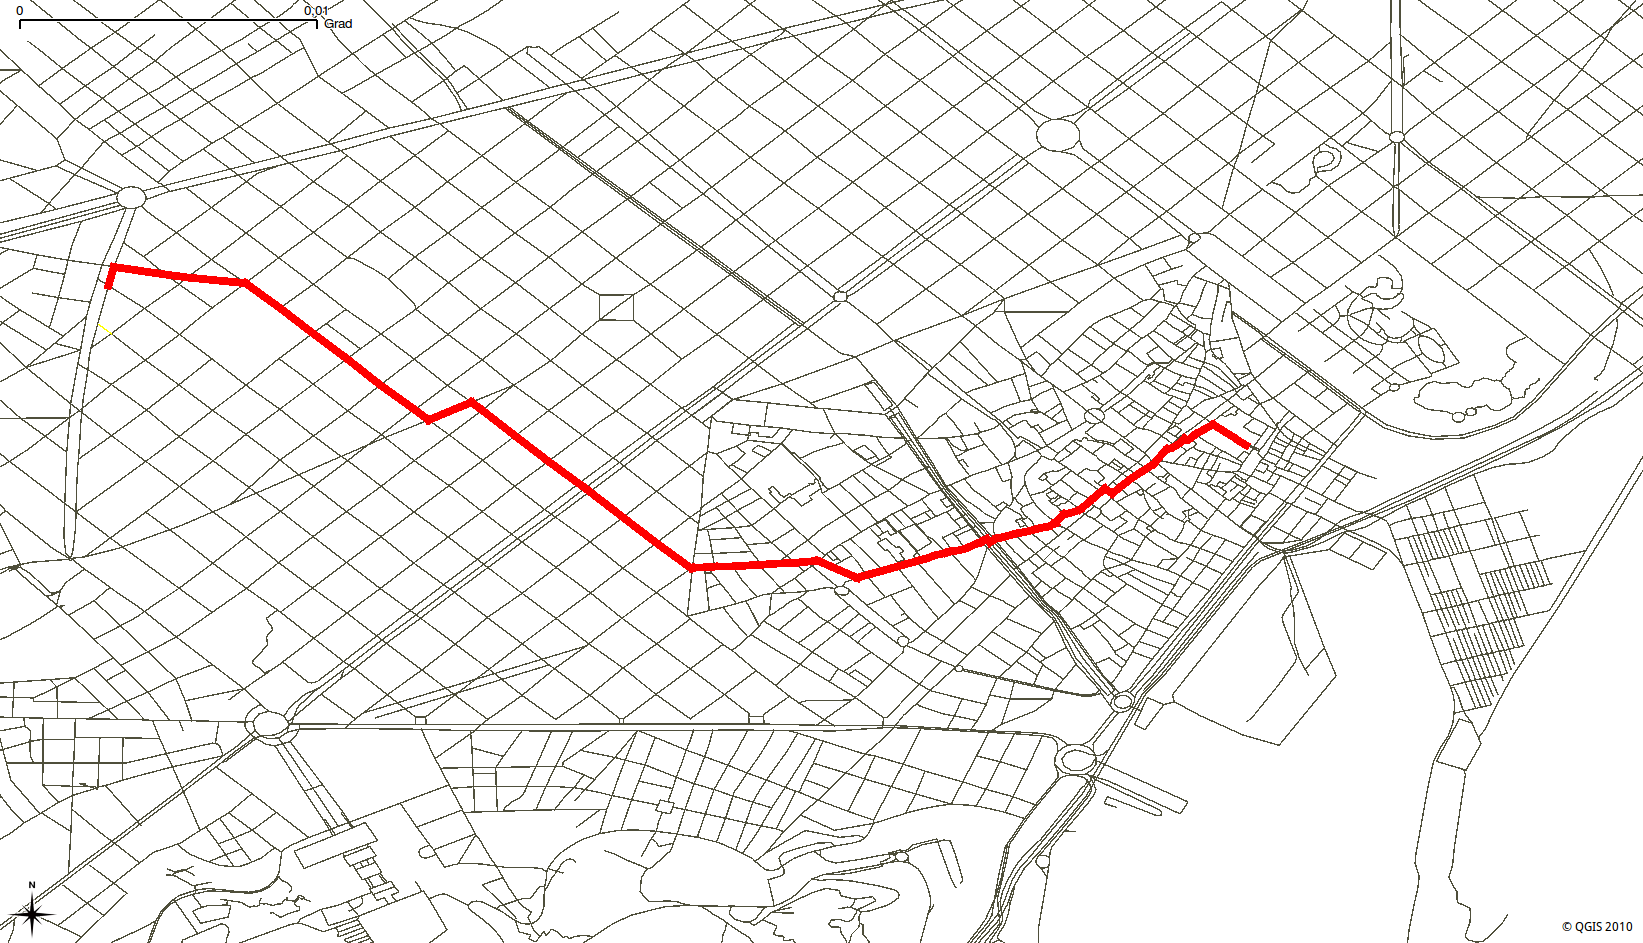
\includegraphics[width=250pt]{route.png}\hfill}


\section{Dijkstra algorithm}

Dijkstra algorithm was the first algorithm implemented in pgRouting. It doesn't require more attributes than source and target ID, and it can distinguish between directed and undirected graphs. You can specify if your network has ``reverse cost'' or not.

\begin{Verbatim}[commandchars=\\\{\}]
\PYG{n}{shortest\PYGZus{}path}\PYG{p}{(} \PYG{k}{sql} \PYG{n+nb}{text}\PYG{p}{,}
                   \PYG{n}{source\PYGZus{}id} \PYG{n+nb}{integer}\PYG{p}{,}
                   \PYG{n}{target\PYGZus{}id} \PYG{n+nb}{integer}\PYG{p}{,}
                   \PYG{n}{directed} \PYG{n+nb}{boolean}\PYG{p}{,}
                   \PYG{n}{has\PYGZus{}reverse\PYGZus{}cost} \PYG{n+nb}{boolean} \PYG{p}{)}
\end{Verbatim}

\begin{notice}{note}{Note:}\begin{itemize}
\item {} 
Source and target IDs are vertex IDs.

\item {} 
Undirected graphs (``directed false'') ignores ``has\_reverse\_cost'' setting

\item {} 
Shortest Path Dijkstra core function

\end{itemize}
\end{notice}


\subsection{Core}

Each algorithm has its core function (implementation), which is the base for its wrapper functions.

\begin{Verbatim}[commandchars=\\\{\}]
\PYG{k}{SELECT} \PYG{o}{*} \PYG{k}{FROM} \PYG{n}{shortest\PYGZus{}path}\PYG{p}{(}\PYG{l+s+s1}{'}
\PYG{l+s+s1}{                SELECT gid as id,}
\PYG{l+s+s1}{                         source::integer,}
\PYG{l+s+s1}{                         target::integer,}
\PYG{l+s+s1}{                         length::double precision as cost}
\PYG{l+s+s1}{                        FROM ways'}\PYG{p}{,}
                \PYG{l+m+mi}{10}\PYG{p}{,} \PYG{l+m+mi}{20}\PYG{p}{,} \PYG{k}{false}\PYG{p}{,} \PYG{k}{false}\PYG{p}{)}\PYG{p}{;}
\end{Verbatim}

\begin{Verbatim}[commandchars=\\\{\}]
 \PYG{n}{vertex\PYGZus{}id} \PYG{o}{\textbar{}} \PYG{n}{edge\PYGZus{}id} \PYG{o}{\textbar{}}        \PYG{n}{cost}
\PYG{c+c1}{-----------+---------+---------------------}
        \PYG{l+m+mi}{10} \PYG{o}{\textbar{}}     \PYG{l+m+mi}{293} \PYG{o}{\textbar{}}  \PYG{l+m+mi}{0}\PYG{p}{.}\PYG{l+m+mi}{0059596293824534}
         \PYG{l+m+mi}{9} \PYG{o}{\textbar{}}    \PYG{l+m+mi}{4632} \PYG{o}{\textbar{}}  \PYG{l+m+mi}{0}\PYG{p}{.}\PYG{l+m+mi}{0846731039249787}
      \PYG{l+m+mi}{3974} \PYG{o}{\textbar{}}    \PYG{l+m+mi}{4633} \PYG{o}{\textbar{}}  \PYG{l+m+mi}{0}\PYG{p}{.}\PYG{l+m+mi}{0765635090514303}
      \PYG{l+m+mi}{2107} \PYG{o}{\textbar{}}    \PYG{l+m+mi}{4634} \PYG{o}{\textbar{}}  \PYG{l+m+mi}{0}\PYG{p}{.}\PYG{l+m+mi}{0763951531894937}
       \PYG{p}{.}\PYG{p}{.}\PYG{p}{.} \PYG{o}{\textbar{}}     \PYG{p}{.}\PYG{p}{.}\PYG{p}{.} \PYG{o}{\textbar{}}  \PYG{p}{.}\PYG{p}{.}\PYG{p}{.}
        \PYG{l+m+mi}{20} \PYG{o}{\textbar{}}      \PYG{o}{-}\PYG{l+m+mi}{1} \PYG{o}{\textbar{}}                   \PYG{l+m+mi}{0}
\PYG{p}{(}\PYG{l+m+mi}{63} \PYG{k}{rows}\PYG{p}{)}
\end{Verbatim}


\subsection{Wrapper}
\paragraph{Wrapper WITHOUT bounding box}

Wrapper functions extend the core functions with transformations, bounding box limitations, etc.. Wrappers can change the format and ordering of the result. They often set default function parameters and make the usage of pgRouting more simple.

\begin{Verbatim}[commandchars=\\\{\}]
\PYG{k}{SELECT} \PYG{n}{gid}\PYG{p}{,} \PYG{n}{AsText}\PYG{p}{(}\PYG{n}{the\PYGZus{}geom}\PYG{p}{)} \PYG{k}{AS} \PYG{n}{the\PYGZus{}geom}
        \PYG{k}{FROM} \PYG{n}{dijkstra\PYGZus{}sp}\PYG{p}{(}\PYG{l+s+s1}{'ways'}\PYG{p}{,} \PYG{l+m+mi}{10}\PYG{p}{,} \PYG{l+m+mi}{20}\PYG{p}{)}\PYG{p}{;}
\end{Verbatim}

\begin{Verbatim}[commandchars=\\\{\}]
  \PYG{n}{gid}   \PYG{o}{\textbar{}}                              \PYG{n}{the\PYGZus{}geom}
\PYG{c+c1}{--------+---------------------------------------------------------------}
    \PYG{l+m+mi}{293} \PYG{o}{\textbar{}} \PYG{n}{MULTILINESTRING}\PYG{p}{(}\PYG{p}{(}\PYG{l+m+mi}{18}\PYG{p}{.}\PYG{l+m+mi}{4074149} \PYG{o}{-}\PYG{l+m+mi}{33}\PYG{p}{.}\PYG{l+m+mi}{9443308}\PYG{p}{,}\PYG{l+m+mi}{18}\PYG{p}{.}\PYG{l+m+mi}{4074019} \PYG{o}{-}\PYG{l+m+mi}{33}\PYG{p}{.}\PYG{l+m+mi}{9443833}\PYG{p}{)}\PYG{p}{)}
   \PYG{l+m+mi}{4632} \PYG{o}{\textbar{}} \PYG{n}{MULTILINESTRING}\PYG{p}{(}\PYG{p}{(}\PYG{l+m+mi}{18}\PYG{p}{.}\PYG{l+m+mi}{4074149} \PYG{o}{-}\PYG{l+m+mi}{33}\PYG{p}{.}\PYG{l+m+mi}{9443308}\PYG{p}{,}\PYG{l+m+mi}{18}\PYG{p}{.}\PYG{l+m+mi}{4077388} \PYG{o}{-}\PYG{l+m+mi}{33}\PYG{p}{.}\PYG{l+m+mi}{9436183}\PYG{p}{)}\PYG{p}{)}
   \PYG{l+m+mi}{4633} \PYG{o}{\textbar{}} \PYG{n}{MULTILINESTRING}\PYG{p}{(}\PYG{p}{(}\PYG{l+m+mi}{18}\PYG{p}{.}\PYG{l+m+mi}{4077388} \PYG{o}{-}\PYG{l+m+mi}{33}\PYG{p}{.}\PYG{l+m+mi}{9436183}\PYG{p}{,}\PYG{l+m+mi}{18}\PYG{p}{.}\PYG{l+m+mi}{4080293} \PYG{o}{-}\PYG{l+m+mi}{33}\PYG{p}{.}\PYG{l+m+mi}{9429733}\PYG{p}{)}\PYG{p}{)}
    \PYG{p}{.}\PYG{p}{.}\PYG{p}{.} \PYG{o}{\textbar{}} \PYG{p}{.}\PYG{p}{.}\PYG{p}{.}
    \PYG{l+m+mi}{762} \PYG{o}{\textbar{}} \PYG{n}{MULTILINESTRING}\PYG{p}{(}\PYG{p}{(}\PYG{l+m+mi}{18}\PYG{p}{.}\PYG{l+m+mi}{4241422} \PYG{o}{-}\PYG{l+m+mi}{33}\PYG{p}{.}\PYG{l+m+mi}{9179275}\PYG{p}{,}\PYG{l+m+mi}{18}\PYG{p}{.}\PYG{l+m+mi}{4237423} \PYG{o}{-}\PYG{l+m+mi}{33}\PYG{p}{.}\PYG{l+m+mi}{9182966}\PYG{p}{)}\PYG{p}{)}
    \PYG{l+m+mi}{761} \PYG{o}{\textbar{}} \PYG{n}{MULTILINESTRING}\PYG{p}{(}\PYG{p}{(}\PYG{l+m+mi}{18}\PYG{p}{.}\PYG{l+m+mi}{4243523} \PYG{o}{-}\PYG{l+m+mi}{33}\PYG{p}{.}\PYG{l+m+mi}{9177154}\PYG{p}{,}\PYG{l+m+mi}{18}\PYG{p}{.}\PYG{l+m+mi}{4241422} \PYG{o}{-}\PYG{l+m+mi}{33}\PYG{p}{.}\PYG{l+m+mi}{9179275}\PYG{p}{)}\PYG{p}{)}
\PYG{p}{(}\PYG{l+m+mi}{62} \PYG{k}{rows}\PYG{p}{)}
\end{Verbatim}
\paragraph{Wrapper WITH bounding box}

You can limit your search area by adding a bounding box. This will improve performance especially for large networks.

\begin{Verbatim}[commandchars=\\\{\}]
\PYG{k}{SELECT} \PYG{n}{gid}\PYG{p}{,} \PYG{n}{AsText}\PYG{p}{(}\PYG{n}{the\PYGZus{}geom}\PYG{p}{)} \PYG{k}{AS} \PYG{n}{the\PYGZus{}geom}
        \PYG{k}{FROM} \PYG{n}{dijkstra\PYGZus{}sp\PYGZus{}delta}\PYG{p}{(}\PYG{l+s+s1}{'ways'}\PYG{p}{,} \PYG{l+m+mi}{10}\PYG{p}{,} \PYG{l+m+mi}{20}\PYG{p}{,} \PYG{l+m+mi}{0}\PYG{p}{.}\PYG{l+m+mi}{1}\PYG{p}{)}\PYG{p}{;}
\end{Verbatim}

\begin{Verbatim}[commandchars=\\\{\}]
   \PYG{n}{gid}  \PYG{o}{\textbar{}} \PYG{n}{the\PYGZus{}geom}
\PYG{c+c1}{--------+---------------------------------------------------------------}
   \PYG{l+m+mi}{293}  \PYG{o}{\textbar{}} \PYG{n}{MULTILINESTRING}\PYG{p}{(}\PYG{p}{(}\PYG{l+m+mi}{18}\PYG{p}{.}\PYG{l+m+mi}{4074149} \PYG{o}{-}\PYG{l+m+mi}{33}\PYG{p}{.}\PYG{l+m+mi}{9443308}\PYG{p}{,}\PYG{l+m+mi}{18}\PYG{p}{.}\PYG{l+m+mi}{4074019} \PYG{o}{-}\PYG{l+m+mi}{33}\PYG{p}{.}\PYG{l+m+mi}{9443833}\PYG{p}{)}\PYG{p}{)}
   \PYG{l+m+mi}{4632} \PYG{o}{\textbar{}} \PYG{n}{MULTILINESTRING}\PYG{p}{(}\PYG{p}{(}\PYG{l+m+mi}{18}\PYG{p}{.}\PYG{l+m+mi}{4074149} \PYG{o}{-}\PYG{l+m+mi}{33}\PYG{p}{.}\PYG{l+m+mi}{9443308}\PYG{p}{,}\PYG{l+m+mi}{18}\PYG{p}{.}\PYG{l+m+mi}{4077388} \PYG{o}{-}\PYG{l+m+mi}{33}\PYG{p}{.}\PYG{l+m+mi}{9436183}\PYG{p}{)}\PYG{p}{)}
   \PYG{l+m+mi}{4633} \PYG{o}{\textbar{}} \PYG{n}{MULTILINESTRING}\PYG{p}{(}\PYG{p}{(}\PYG{l+m+mi}{18}\PYG{p}{.}\PYG{l+m+mi}{4077388} \PYG{o}{-}\PYG{l+m+mi}{33}\PYG{p}{.}\PYG{l+m+mi}{9436183}\PYG{p}{,}\PYG{l+m+mi}{18}\PYG{p}{.}\PYG{l+m+mi}{4080293} \PYG{o}{-}\PYG{l+m+mi}{33}\PYG{p}{.}\PYG{l+m+mi}{9429733}\PYG{p}{)}\PYG{p}{)}
   \PYG{p}{.}\PYG{p}{.}\PYG{p}{.}  \PYG{o}{\textbar{}} \PYG{p}{.}\PYG{p}{.}\PYG{p}{.}
   \PYG{l+m+mi}{762}  \PYG{o}{\textbar{}} \PYG{n}{MULTILINESTRING}\PYG{p}{(}\PYG{p}{(}\PYG{l+m+mi}{18}\PYG{p}{.}\PYG{l+m+mi}{4241422} \PYG{o}{-}\PYG{l+m+mi}{33}\PYG{p}{.}\PYG{l+m+mi}{9179275}\PYG{p}{,}\PYG{l+m+mi}{18}\PYG{p}{.}\PYG{l+m+mi}{4237423} \PYG{o}{-}\PYG{l+m+mi}{33}\PYG{p}{.}\PYG{l+m+mi}{9182966}\PYG{p}{)}\PYG{p}{)}
   \PYG{l+m+mi}{761} \PYG{o}{\textbar{}} \PYG{n}{MULTILINESTRING}\PYG{p}{(}\PYG{p}{(}\PYG{l+m+mi}{18}\PYG{p}{.}\PYG{l+m+mi}{4243523} \PYG{o}{-}\PYG{l+m+mi}{33}\PYG{p}{.}\PYG{l+m+mi}{9177154}\PYG{p}{,}\PYG{l+m+mi}{18}\PYG{p}{.}\PYG{l+m+mi}{4241422} \PYG{o}{-}\PYG{l+m+mi}{33}\PYG{p}{.}\PYG{l+m+mi}{9179275}\PYG{p}{)}\PYG{p}{)}
\PYG{p}{(}\PYG{l+m+mi}{62} \PYG{k}{rows}\PYG{p}{)}
\end{Verbatim}

\begin{notice}{warning}{Warning:}
The projection of OSM data is ``degree'', so we set a bounding box containing start and end vertex plus a 0.1 degree buffer for example.
\end{notice}


\section{A-Star algorithm}

A-Star algorithm is another well-known routing algorithm. It adds geographical information to source and target of each network link. This enables the shortest path search to prefer links which are closer to the target of the search.


\subsection{Prerequisites}

For A-Star you need to prepare your network table and add latitute/longitude columns (x1, y1 and x2, y2) and calculate their values.

\begin{Verbatim}[commandchars=\\\{\}]
\PYG{k}{ALTER} \PYG{k}{TABLE} \PYG{n}{ways} \PYG{k}{ADD} \PYG{k}{COLUMN} \PYG{n}{x1} \PYG{n}{double} \PYG{k}{precision}\PYG{p}{;}
\PYG{k}{ALTER} \PYG{k}{TABLE} \PYG{n}{ways} \PYG{k}{ADD} \PYG{k}{COLUMN} \PYG{n}{y1} \PYG{n}{double} \PYG{k}{precision}\PYG{p}{;}
\PYG{k}{ALTER} \PYG{k}{TABLE} \PYG{n}{ways} \PYG{k}{ADD} \PYG{k}{COLUMN} \PYG{n}{x2} \PYG{n}{double} \PYG{k}{precision}\PYG{p}{;}
\PYG{k}{ALTER} \PYG{k}{TABLE} \PYG{n}{ways} \PYG{k}{ADD} \PYG{k}{COLUMN} \PYG{n}{y2} \PYG{n}{double} \PYG{k}{precision}\PYG{p}{;}

\PYG{k}{UPDATE} \PYG{n}{ways} \PYG{k}{SET} \PYG{n}{x1} \PYG{o}{=} \PYG{n}{x}\PYG{p}{(}\PYG{n}{startpoint}\PYG{p}{(}\PYG{n}{the\PYGZus{}geom}\PYG{p}{)}\PYG{p}{)}\PYG{p}{;}
\PYG{k}{UPDATE} \PYG{n}{ways} \PYG{k}{SET} \PYG{n}{y1} \PYG{o}{=} \PYG{n}{y}\PYG{p}{(}\PYG{n}{startpoint}\PYG{p}{(}\PYG{n}{the\PYGZus{}geom}\PYG{p}{)}\PYG{p}{)}\PYG{p}{;}

\PYG{k}{UPDATE} \PYG{n}{ways} \PYG{k}{SET} \PYG{n}{x2} \PYG{o}{=} \PYG{n}{x}\PYG{p}{(}\PYG{n}{endpoint}\PYG{p}{(}\PYG{n}{the\PYGZus{}geom}\PYG{p}{)}\PYG{p}{)}\PYG{p}{;}
\PYG{k}{UPDATE} \PYG{n}{ways} \PYG{k}{SET} \PYG{n}{y2} \PYG{o}{=} \PYG{n}{y}\PYG{p}{(}\PYG{n}{endpoint}\PYG{p}{(}\PYG{n}{the\PYGZus{}geom}\PYG{p}{)}\PYG{p}{)}\PYG{p}{;}

\PYG{k}{UPDATE} \PYG{n}{ways} \PYG{k}{SET} \PYG{n}{x1} \PYG{o}{=} \PYG{n}{x}\PYG{p}{(}\PYG{n}{PointN}\PYG{p}{(}\PYG{n}{the\PYGZus{}geom}\PYG{p}{,} \PYG{l+m+mi}{1}\PYG{p}{)}\PYG{p}{)}\PYG{p}{;}
\PYG{k}{UPDATE} \PYG{n}{ways} \PYG{k}{SET} \PYG{n}{y1} \PYG{o}{=} \PYG{n}{y}\PYG{p}{(}\PYG{n}{PointN}\PYG{p}{(}\PYG{n}{the\PYGZus{}geom}\PYG{p}{,} \PYG{l+m+mi}{1}\PYG{p}{)}\PYG{p}{)}\PYG{p}{;}

\PYG{k}{UPDATE} \PYG{n}{ways} \PYG{k}{SET} \PYG{n}{x2} \PYG{o}{=} \PYG{n}{x}\PYG{p}{(}\PYG{n}{PointN}\PYG{p}{(}\PYG{n}{the\PYGZus{}geom}\PYG{p}{,} \PYG{n}{NumPoints}\PYG{p}{(}\PYG{n}{the\PYGZus{}geom}\PYG{p}{)}\PYG{p}{)}\PYG{p}{)}\PYG{p}{;}
\PYG{k}{UPDATE} \PYG{n}{ways} \PYG{k}{SET} \PYG{n}{y2} \PYG{o}{=} \PYG{n}{y}\PYG{p}{(}\PYG{n}{PointN}\PYG{p}{(}\PYG{n}{the\PYGZus{}geom}\PYG{p}{,} \PYG{n}{NumPoints}\PYG{p}{(}\PYG{n}{the\PYGZus{}geom}\PYG{p}{)}\PYG{p}{)}\PYG{p}{)}\PYG{p}{;}
\end{Verbatim}

\begin{notice}{note}{Note:}
``endpoint()'' function fails for some versions of PostgreSQL (ie. 8.2.5, 8.1.9). A workaround for that problem is using the ``PointN()'' function instead:
\end{notice}


\subsection{Core}

Shortest Path A-Star function is very similar to the Dijkstra function, though it prefers links that are close to the target of the search. The heuristics of this search are predefined, so you need to recompile pgRouting if you want to make changes to the heuristic function itself.

\begin{Verbatim}[commandchars=\\\{\}]
\PYG{n}{shortest\PYGZus{}path\PYGZus{}astar}\PYG{p}{(} \PYG{k}{sql} \PYG{n+nb}{text}\PYG{p}{,}
                   \PYG{n}{source\PYGZus{}id} \PYG{n+nb}{integer}\PYG{p}{,}
                   \PYG{n}{target\PYGZus{}id} \PYG{n+nb}{integer}\PYG{p}{,}
                   \PYG{n}{directed} \PYG{n+nb}{boolean}\PYG{p}{,}
                   \PYG{n}{has\PYGZus{}reverse\PYGZus{}cost} \PYG{n+nb}{boolean} \PYG{p}{)}
\end{Verbatim}

\begin{notice}{note}{Note:}\begin{itemize}
\item {} 
Source and target IDs are vertex IDs.

\item {} 
Undirected graphs (``directed false'') ignores ``has\_reverse\_cost'' setting

\item {} 
Example of A-Star core function

\end{itemize}
\end{notice}

\begin{Verbatim}[commandchars=\\\{\}]
\PYG{k}{SELECT} \PYG{o}{*} \PYG{k}{FROM} \PYG{n}{shortest\PYGZus{}path\PYGZus{}astar}\PYG{p}{(}\PYG{l+s+s1}{'}
\PYG{l+s+s1}{                SELECT gid as id,}
\PYG{l+s+s1}{                         source::integer,}
\PYG{l+s+s1}{                         target::integer,}
\PYG{l+s+s1}{                         length::double precision as cost,}
\PYG{l+s+s1}{                         x1, y1, x2, y2}
\PYG{l+s+s1}{                        FROM ways'}\PYG{p}{,}
                \PYG{l+m+mi}{10}\PYG{p}{,} \PYG{l+m+mi}{20}\PYG{p}{,} \PYG{k}{false}\PYG{p}{,} \PYG{k}{false}\PYG{p}{)}\PYG{p}{;}
\end{Verbatim}

\begin{Verbatim}[commandchars=\\\{\}]
\PYG{n}{vertex\PYGZus{}id} \PYG{o}{\textbar{}} \PYG{n}{edge\PYGZus{}id} \PYG{o}{\textbar{}}        \PYG{n}{cost}
\PYG{c+c1}{-----------+---------+---------------------}
       \PYG{l+m+mi}{10} \PYG{o}{\textbar{}}     \PYG{l+m+mi}{293} \PYG{o}{\textbar{}}  \PYG{l+m+mi}{0}\PYG{p}{.}\PYG{l+m+mi}{0059596293824534}
        \PYG{l+m+mi}{9} \PYG{o}{\textbar{}}    \PYG{l+m+mi}{4632} \PYG{o}{\textbar{}}  \PYG{l+m+mi}{0}\PYG{p}{.}\PYG{l+m+mi}{0846731039249787}
     \PYG{l+m+mi}{3974} \PYG{o}{\textbar{}}    \PYG{l+m+mi}{4633} \PYG{o}{\textbar{}}  \PYG{l+m+mi}{0}\PYG{p}{.}\PYG{l+m+mi}{0765635090514303}
      \PYG{p}{.}\PYG{p}{.}\PYG{p}{.} \PYG{o}{\textbar{}}     \PYG{p}{.}\PYG{p}{.}\PYG{p}{.} \PYG{o}{\textbar{}}  \PYG{p}{.}\PYG{p}{.}\PYG{p}{.}
       \PYG{l+m+mi}{20} \PYG{o}{\textbar{}}      \PYG{o}{-}\PYG{l+m+mi}{1} \PYG{o}{\textbar{}}                   \PYG{l+m+mi}{0}
\PYG{p}{(}\PYG{l+m+mi}{63} \PYG{k}{rows}\PYG{p}{)}
\end{Verbatim}


\subsection{Wrapper}
\paragraph{Wrapper function WITH bounding box}

Wrapper functions extend the core functions with transformations, bounding box limitations, etc..

\begin{Verbatim}[commandchars=\\\{\}]
\PYG{k}{SELECT} \PYG{n}{gid}\PYG{p}{,} \PYG{n}{AsText}\PYG{p}{(}\PYG{n}{the\PYGZus{}geom}\PYG{p}{)} \PYG{k}{AS} \PYG{n}{the\PYGZus{}geom}
        \PYG{k}{FROM} \PYG{n}{astar\PYGZus{}sp\PYGZus{}delta}\PYG{p}{(}\PYG{l+s+s1}{'ways'}\PYG{p}{,} \PYG{l+m+mi}{10}\PYG{p}{,} \PYG{l+m+mi}{20}\PYG{p}{,} \PYG{l+m+mi}{0}\PYG{p}{.}\PYG{l+m+mi}{1}\PYG{p}{)}\PYG{p}{;}
\end{Verbatim}

\begin{Verbatim}[commandchars=\\\{\}]
  \PYG{n}{gid}   \PYG{o}{\textbar{}}                              \PYG{n}{the\PYGZus{}geom}
\PYG{c+c1}{--------+---------------------------------------------------------------}
    \PYG{l+m+mi}{293} \PYG{o}{\textbar{}} \PYG{n}{MULTILINESTRING}\PYG{p}{(}\PYG{p}{(}\PYG{l+m+mi}{18}\PYG{p}{.}\PYG{l+m+mi}{4074149} \PYG{o}{-}\PYG{l+m+mi}{33}\PYG{p}{.}\PYG{l+m+mi}{9443308}\PYG{p}{,}\PYG{l+m+mi}{18}\PYG{p}{.}\PYG{l+m+mi}{4074019} \PYG{o}{-}\PYG{l+m+mi}{33}\PYG{p}{.}\PYG{l+m+mi}{9443833}\PYG{p}{)}\PYG{p}{)}
   \PYG{l+m+mi}{4632} \PYG{o}{\textbar{}} \PYG{n}{MULTILINESTRING}\PYG{p}{(}\PYG{p}{(}\PYG{l+m+mi}{18}\PYG{p}{.}\PYG{l+m+mi}{4074149} \PYG{o}{-}\PYG{l+m+mi}{33}\PYG{p}{.}\PYG{l+m+mi}{9443308}\PYG{p}{,}\PYG{l+m+mi}{18}\PYG{p}{.}\PYG{l+m+mi}{4077388} \PYG{o}{-}\PYG{l+m+mi}{33}\PYG{p}{.}\PYG{l+m+mi}{9436183}\PYG{p}{)}\PYG{p}{)}
   \PYG{l+m+mi}{4633} \PYG{o}{\textbar{}} \PYG{n}{MULTILINESTRING}\PYG{p}{(}\PYG{p}{(}\PYG{l+m+mi}{18}\PYG{p}{.}\PYG{l+m+mi}{4077388} \PYG{o}{-}\PYG{l+m+mi}{33}\PYG{p}{.}\PYG{l+m+mi}{9436183}\PYG{p}{,}\PYG{l+m+mi}{18}\PYG{p}{.}\PYG{l+m+mi}{4080293} \PYG{o}{-}\PYG{l+m+mi}{33}\PYG{p}{.}\PYG{l+m+mi}{9429733}\PYG{p}{)}\PYG{p}{)}
    \PYG{p}{.}\PYG{p}{.}\PYG{p}{.} \PYG{o}{\textbar{}} \PYG{p}{.}\PYG{p}{.}\PYG{p}{.}
    \PYG{l+m+mi}{762} \PYG{o}{\textbar{}} \PYG{n}{MULTILINESTRING}\PYG{p}{(}\PYG{p}{(}\PYG{l+m+mi}{18}\PYG{p}{.}\PYG{l+m+mi}{4241422} \PYG{o}{-}\PYG{l+m+mi}{33}\PYG{p}{.}\PYG{l+m+mi}{9179275}\PYG{p}{,}\PYG{l+m+mi}{18}\PYG{p}{.}\PYG{l+m+mi}{4237423} \PYG{o}{-}\PYG{l+m+mi}{33}\PYG{p}{.}\PYG{l+m+mi}{9182966}\PYG{p}{)}\PYG{p}{)}
    \PYG{l+m+mi}{761} \PYG{o}{\textbar{}} \PYG{n}{MULTILINESTRING}\PYG{p}{(}\PYG{p}{(}\PYG{l+m+mi}{18}\PYG{p}{.}\PYG{l+m+mi}{4243523} \PYG{o}{-}\PYG{l+m+mi}{33}\PYG{p}{.}\PYG{l+m+mi}{9177154}\PYG{p}{,}\PYG{l+m+mi}{18}\PYG{p}{.}\PYG{l+m+mi}{4241422} \PYG{o}{-}\PYG{l+m+mi}{33}\PYG{p}{.}\PYG{l+m+mi}{9179275}\PYG{p}{)}\PYG{p}{)}
\PYG{p}{(}\PYG{l+m+mi}{62} \PYG{k}{rows}\PYG{p}{)}
\end{Verbatim}

\begin{notice}{note}{Note:}
There is currently no wrapper function for A-Star without bounding box, since bounding boxes are very useful to increase performance. If you don't need a bounding box Dijkstra will be enough anyway.
\end{notice}

\begin{notice}{warning}{Warning:}
The projection of OSM data is ``degree'', so we set a bounding box containing start and end vertex plus a 0.1 degree buffer for example.
\end{notice}


\section{Shooting-Star algorithm}

Shooting-Star algorithm is the latest of pgRouting shortest path algorithms. Its speciality is that it routes from link to link, not from vertex to vertex as Dijkstra and A-Star algorithms do. This makes it possible to define relations between links for example, and it solves some other vertex-based algorithm issues like ``parallel links'', which have same source and target but different costs.


\subsection{Prerequisites}

For Shooting-Star you need to prepare your network table and add the ``reverse\_cost'' and ``to\_cost'' column. Like A-Star this algorithm also has a heuristic function, which prefers links closer to the target of the search.

\begin{Verbatim}[commandchars=\\\{\}]
\PYG{k}{ALTER} \PYG{k}{TABLE} \PYG{n}{ways} \PYG{k}{ADD} \PYG{k}{COLUMN} \PYG{n}{reverse\PYGZus{}cost} \PYG{n}{double} \PYG{k}{precision}\PYG{p}{;}
\PYG{k}{UPDATE} \PYG{n}{ways} \PYG{k}{SET} \PYG{n}{reverse\PYGZus{}cost} \PYG{o}{=} \PYG{k}{length}\PYG{p}{;}

\PYG{k}{ALTER} \PYG{k}{TABLE} \PYG{n}{ways} \PYG{k}{ADD} \PYG{k}{COLUMN} \PYG{n}{to\PYGZus{}cost} \PYG{n}{double} \PYG{k}{precision}\PYG{p}{;}

\PYG{k}{ALTER} \PYG{k}{TABLE} \PYG{n}{ways} \PYG{k}{ADD} \PYG{k}{COLUMN} \PYG{k}{rule} \PYG{n+nb}{text}\PYG{p}{;}
\end{Verbatim}
\paragraph{Shooting-Star algorithm introduces two new attributes}
\begin{itemize}
\item {} 
\textbf{rule}: a string with a comma separated list of edge IDs, which describes a rule for turning restriction (if you came along these edges, you can pass through the current one only with the cost stated in to\_cost column)

\item {} 
\textbf{to\_cost}: a cost of a restricted passage (can be very high in a case of turn restriction or comparable with an edge cost in a case of traffic light)

\end{itemize}

\begin{Verbatim}[commandchars=\\\{\}]
\PYG{n}{shortest\PYGZus{}path\PYGZus{}shooting\PYGZus{}star}\PYG{p}{(} \PYG{k}{sql} \PYG{n+nb}{text}\PYG{p}{,}
                   \PYG{n}{source\PYGZus{}id} \PYG{n+nb}{integer}\PYG{p}{,}
                   \PYG{n}{target\PYGZus{}id} \PYG{n+nb}{integer}\PYG{p}{,}
                   \PYG{n}{directed} \PYG{n+nb}{boolean}\PYG{p}{,}
                   \PYG{n}{has\PYGZus{}reverse\PYGZus{}cost} \PYG{n+nb}{boolean} \PYG{p}{)}
\end{Verbatim}

\begin{notice}{note}{Note:}\begin{itemize}
\item {} 
Source and target IDs are link IDs.

\item {} 
Undirected graphs (``directed false'') ignores ``has\_reverse\_cost'' setting

\item {} 
Example for Shooting-Star ``rule''

\end{itemize}
\end{notice}

\begin{notice}{warning}{Warning:}
Shooting* algorithm calculates a path from edge to edge (not from vertex to vertex). Column vertex\_id contains start vertex of an edge from column edge\_id.
\end{notice}

To describe turn restrictions:

\begin{Verbatim}[commandchars=\\\{\}]
 \PYG{n}{gid} \PYG{o}{\textbar{}} \PYG{k}{source} \PYG{o}{\textbar{}} \PYG{n}{target} \PYG{o}{\textbar{}} \PYG{n}{cost} \PYG{o}{\textbar{}} \PYG{n}{x1} \PYG{o}{\textbar{}} \PYG{n}{y1} \PYG{o}{\textbar{}} \PYG{n}{x2} \PYG{o}{\textbar{}} \PYG{n}{y2} \PYG{o}{\textbar{}} \PYG{n}{to\PYGZus{}cost} \PYG{o}{\textbar{}} \PYG{k}{rule}
\PYG{c+c1}{-----+--------+--------+------+----+----+----+----+---------+------}
  \PYG{l+m+mi}{12} \PYG{o}{\textbar{}}      \PYG{l+m+mi}{3} \PYG{o}{\textbar{}}     \PYG{l+m+mi}{10} \PYG{o}{\textbar{}}    \PYG{l+m+mi}{2} \PYG{o}{\textbar{}}  \PYG{l+m+mi}{4} \PYG{o}{\textbar{}}  \PYG{l+m+mi}{3} \PYG{o}{\textbar{}}  \PYG{l+m+mi}{4} \PYG{o}{\textbar{}}  \PYG{l+m+mi}{5} \PYG{o}{\textbar{}}    \PYG{l+m+mi}{1000} \PYG{o}{\textbar{}} \PYG{l+m+mi}{14}
\end{Verbatim}

... means that the cost of going from edge 14 to edge 12 is 1000, and

\begin{Verbatim}[commandchars=\\\{\}]
 \PYG{n}{gid} \PYG{o}{\textbar{}} \PYG{k}{source} \PYG{o}{\textbar{}} \PYG{n}{target} \PYG{o}{\textbar{}} \PYG{n}{cost} \PYG{o}{\textbar{}} \PYG{n}{x1} \PYG{o}{\textbar{}} \PYG{n}{y1} \PYG{o}{\textbar{}} \PYG{n}{x2} \PYG{o}{\textbar{}} \PYG{n}{y2} \PYG{o}{\textbar{}} \PYG{n}{to\PYGZus{}cost} \PYG{o}{\textbar{}} \PYG{k}{rule}
\PYG{c+c1}{-----+--------+--------+------+----+----+----+----+---------+------}
  \PYG{l+m+mi}{12} \PYG{o}{\textbar{}}      \PYG{l+m+mi}{3} \PYG{o}{\textbar{}}     \PYG{l+m+mi}{10} \PYG{o}{\textbar{}}    \PYG{l+m+mi}{2} \PYG{o}{\textbar{}}  \PYG{l+m+mi}{4} \PYG{o}{\textbar{}}  \PYG{l+m+mi}{3} \PYG{o}{\textbar{}}  \PYG{l+m+mi}{4} \PYG{o}{\textbar{}}  \PYG{l+m+mi}{5} \PYG{o}{\textbar{}}    \PYG{l+m+mi}{1000} \PYG{o}{\textbar{}} \PYG{l+m+mi}{14}\PYG{p}{,} \PYG{l+m+mi}{4}
\end{Verbatim}

... means that the cost of going from edge 14 to edge 12 through edge 4 is 1000.

If you need multiple restrictions for a given edge then you have to add multiple records for that edge each with a separate restriction.

\begin{Verbatim}[commandchars=\\\{\}]
 \PYG{n}{gid} \PYG{o}{\textbar{}} \PYG{k}{source} \PYG{o}{\textbar{}} \PYG{n}{target} \PYG{o}{\textbar{}} \PYG{n}{cost} \PYG{o}{\textbar{}} \PYG{n}{x1} \PYG{o}{\textbar{}} \PYG{n}{y1} \PYG{o}{\textbar{}} \PYG{n}{x2} \PYG{o}{\textbar{}} \PYG{n}{y2} \PYG{o}{\textbar{}} \PYG{n}{to\PYGZus{}cost} \PYG{o}{\textbar{}} \PYG{k}{rule}
\PYG{c+c1}{-----+--------+--------+------+----+----+----+----+---------+------}
  \PYG{l+m+mi}{11} \PYG{o}{\textbar{}}      \PYG{l+m+mi}{3} \PYG{o}{\textbar{}}     \PYG{l+m+mi}{10} \PYG{o}{\textbar{}}    \PYG{l+m+mi}{2} \PYG{o}{\textbar{}}  \PYG{l+m+mi}{4} \PYG{o}{\textbar{}}  \PYG{l+m+mi}{3} \PYG{o}{\textbar{}}  \PYG{l+m+mi}{4} \PYG{o}{\textbar{}}  \PYG{l+m+mi}{5} \PYG{o}{\textbar{}}    \PYG{l+m+mi}{1000} \PYG{o}{\textbar{}} \PYG{l+m+mi}{4}
  \PYG{l+m+mi}{11} \PYG{o}{\textbar{}}      \PYG{l+m+mi}{3} \PYG{o}{\textbar{}}     \PYG{l+m+mi}{10} \PYG{o}{\textbar{}}    \PYG{l+m+mi}{2} \PYG{o}{\textbar{}}  \PYG{l+m+mi}{4} \PYG{o}{\textbar{}}  \PYG{l+m+mi}{3} \PYG{o}{\textbar{}}  \PYG{l+m+mi}{4} \PYG{o}{\textbar{}}  \PYG{l+m+mi}{5} \PYG{o}{\textbar{}}    \PYG{l+m+mi}{1000} \PYG{o}{\textbar{}} \PYG{l+m+mi}{12}
\end{Verbatim}

... means that the cost of going from either edge 4 or 12 to edge 11 is 1000. And then you always need to order your data by gid when you load it to a shortest path function..


\subsection{Core}

\begin{Verbatim}[commandchars=\\\{\}]
\PYG{k}{SELECT} \PYG{o}{*} \PYG{k}{FROM} \PYG{n}{shortest\PYGZus{}path\PYGZus{}shooting\PYGZus{}star}\PYG{p}{(}\PYG{l+s+s1}{'}
\PYG{l+s+s1}{                SELECT gid as id,}
\PYG{l+s+s1}{                         source::integer,}
\PYG{l+s+s1}{                         target::integer,}
\PYG{l+s+s1}{                         length::double precision as cost,}
\PYG{l+s+s1}{                         x1, y1, x2, y2,}
\PYG{l+s+s1}{                         rule, to\PYGZus{}cost}
\PYG{l+s+s1}{                        FROM ways'}\PYG{p}{,}
                \PYG{l+m+mi}{293}\PYG{p}{,} \PYG{l+m+mi}{761}\PYG{p}{,} \PYG{k}{false}\PYG{p}{,} \PYG{k}{false}\PYG{p}{)}\PYG{p}{;}
\end{Verbatim}

\begin{Verbatim}[commandchars=\\\{\}]
 \PYG{n}{vertex\PYGZus{}id} \PYG{o}{\textbar{}} \PYG{n}{edge\PYGZus{}id} \PYG{o}{\textbar{}}        \PYG{n}{cost}
\PYG{c+c1}{-----------+---------+---------------------}
      \PYG{l+m+mi}{4232} \PYG{o}{\textbar{}}     \PYG{l+m+mi}{293} \PYG{o}{\textbar{}}  \PYG{l+m+mi}{0}\PYG{p}{.}\PYG{l+m+mi}{0059596293824534}
      \PYG{l+m+mi}{3144} \PYG{o}{\textbar{}}     \PYG{l+m+mi}{293} \PYG{o}{\textbar{}}  \PYG{l+m+mi}{0}\PYG{p}{.}\PYG{l+m+mi}{0059596293824534}
      \PYG{l+m+mi}{4232} \PYG{o}{\textbar{}}    \PYG{l+m+mi}{4632} \PYG{o}{\textbar{}}  \PYG{l+m+mi}{0}\PYG{p}{.}\PYG{l+m+mi}{0846731039249787}
       \PYG{p}{.}\PYG{p}{.}\PYG{p}{.} \PYG{o}{\textbar{}}     \PYG{p}{.}\PYG{p}{.}\PYG{p}{.} \PYG{o}{\textbar{}}  \PYG{p}{.}\PYG{p}{.}\PYG{p}{.}
        \PYG{l+m+mi}{51} \PYG{o}{\textbar{}}     \PYG{l+m+mi}{761} \PYG{o}{\textbar{}}  \PYG{l+m+mi}{0}\PYG{p}{.}\PYG{l+m+mi}{0305298478239596}
\PYG{p}{(}\PYG{l+m+mi}{63} \PYG{k}{rows}\PYG{p}{)}
\end{Verbatim}


\subsection{Wrapper}

Wrapper functions extend the core functions with transformations, bounding box limitations, etc..

\begin{Verbatim}[commandchars=\\\{\}]
\PYG{k}{SELECT} \PYG{n}{gid}\PYG{p}{,} \PYG{n}{AsText}\PYG{p}{(}\PYG{n}{the\PYGZus{}geom}\PYG{p}{)} \PYG{k}{AS} \PYG{n}{the\PYGZus{}geom}
        \PYG{k}{FROM} \PYG{n}{shootingstar\PYGZus{}sp}\PYG{p}{(}\PYG{l+s+s1}{'ways'}\PYG{p}{,} \PYG{l+m+mi}{293}\PYG{p}{,} \PYG{l+m+mi}{761}\PYG{p}{,} \PYG{l+m+mi}{0}\PYG{p}{.}\PYG{l+m+mi}{1}\PYG{p}{,} \PYG{l+s+s1}{'length'}\PYG{p}{,} \PYG{k}{true}\PYG{p}{,} \PYG{k}{true}\PYG{p}{)}\PYG{p}{;}
\end{Verbatim}

\begin{Verbatim}[commandchars=\\\{\}]
  \PYG{n}{gid}   \PYG{o}{\textbar{}}                              \PYG{n}{the\PYGZus{}geom}
\PYG{c+c1}{--------+---------------------------------------------------------------}
    \PYG{l+m+mi}{293} \PYG{o}{\textbar{}} \PYG{n}{MULTILINESTRING}\PYG{p}{(}\PYG{p}{(}\PYG{l+m+mi}{18}\PYG{p}{.}\PYG{l+m+mi}{4074149} \PYG{o}{-}\PYG{l+m+mi}{33}\PYG{p}{.}\PYG{l+m+mi}{9443308}\PYG{p}{,}\PYG{l+m+mi}{18}\PYG{p}{.}\PYG{l+m+mi}{4074019} \PYG{o}{-}\PYG{l+m+mi}{33}\PYG{p}{.}\PYG{l+m+mi}{9443833}\PYG{p}{)}\PYG{p}{)}
    \PYG{l+m+mi}{293} \PYG{o}{\textbar{}} \PYG{n}{MULTILINESTRING}\PYG{p}{(}\PYG{p}{(}\PYG{l+m+mi}{18}\PYG{p}{.}\PYG{l+m+mi}{4074149} \PYG{o}{-}\PYG{l+m+mi}{33}\PYG{p}{.}\PYG{l+m+mi}{9443308}\PYG{p}{,}\PYG{l+m+mi}{18}\PYG{p}{.}\PYG{l+m+mi}{4074019} \PYG{o}{-}\PYG{l+m+mi}{33}\PYG{p}{.}\PYG{l+m+mi}{9443833}\PYG{p}{)}\PYG{p}{)}
   \PYG{l+m+mi}{4632} \PYG{o}{\textbar{}} \PYG{n}{MULTILINESTRING}\PYG{p}{(}\PYG{p}{(}\PYG{l+m+mi}{18}\PYG{p}{.}\PYG{l+m+mi}{4074149} \PYG{o}{-}\PYG{l+m+mi}{33}\PYG{p}{.}\PYG{l+m+mi}{9443308}\PYG{p}{,}\PYG{l+m+mi}{18}\PYG{p}{.}\PYG{l+m+mi}{4077388} \PYG{o}{-}\PYG{l+m+mi}{33}\PYG{p}{.}\PYG{l+m+mi}{9436183}\PYG{p}{)}\PYG{p}{)}
    \PYG{p}{.}\PYG{p}{.}\PYG{p}{.} \PYG{o}{\textbar{}} \PYG{p}{.}\PYG{p}{.}\PYG{p}{.}
    \PYG{l+m+mi}{762} \PYG{o}{\textbar{}} \PYG{n}{MULTILINESTRING}\PYG{p}{(}\PYG{p}{(}\PYG{l+m+mi}{18}\PYG{p}{.}\PYG{l+m+mi}{4241422} \PYG{o}{-}\PYG{l+m+mi}{33}\PYG{p}{.}\PYG{l+m+mi}{9179275}\PYG{p}{,}\PYG{l+m+mi}{18}\PYG{p}{.}\PYG{l+m+mi}{4237423} \PYG{o}{-}\PYG{l+m+mi}{33}\PYG{p}{.}\PYG{l+m+mi}{9182966}\PYG{p}{)}\PYG{p}{)}
    \PYG{l+m+mi}{761} \PYG{o}{\textbar{}} \PYG{n}{MULTILINESTRING}\PYG{p}{(}\PYG{p}{(}\PYG{l+m+mi}{18}\PYG{p}{.}\PYG{l+m+mi}{4243523} \PYG{o}{-}\PYG{l+m+mi}{33}\PYG{p}{.}\PYG{l+m+mi}{9177154}\PYG{p}{,}\PYG{l+m+mi}{18}\PYG{p}{.}\PYG{l+m+mi}{4241422} \PYG{o}{-}\PYG{l+m+mi}{33}\PYG{p}{.}\PYG{l+m+mi}{9179275}\PYG{p}{)}\PYG{p}{)}
\PYG{p}{(}\PYG{l+m+mi}{62} \PYG{k}{rows}\PYG{p}{)}
\end{Verbatim}

\begin{notice}{note}{Note:}
There is currently no wrapper function for A-Star without bounding box, since bounding boxes are very useful to increase performance. If you don't need a bounding box Dijkstra will be enough anyway.
\end{notice}

\begin{notice}{warning}{Warning:}
The projection of OSM data is ``degree'', so we set a bounding box containing start and end vertex plus a 0.1 degree buffer for example.
\end{notice}

\resetcurrentobjects
\hypertarget{--doc-chapters/advanced}{}

\chapter{Advanced usage of pgRouting (bonus chapter)}

An ordinary shortest path query with result usualy looks like this:

\begin{Verbatim}[commandchars=\\\{\}]
\PYG{k}{SELECT} \PYG{o}{*} \PYG{k}{FROM} \PYG{n}{shortest\PYGZus{}path\PYGZus{}shooting\PYGZus{}star}\PYG{p}{(}
        \PYG{l+s+s1}{'SELECT gid as id, source, target, length as cost, x1, y1, x2, y2, rule,}
\PYG{l+s+s1}{        to\PYGZus{}cost, reverse\PYGZus{}cost FROM ways'}\PYG{p}{,} \PYG{l+m+mi}{1955}\PYG{p}{,} \PYG{l+m+mi}{5787}\PYG{p}{,} \PYG{k}{true}\PYG{p}{,} \PYG{k}{true}\PYG{p}{)}\PYG{p}{;}
\end{Verbatim}

Query result:

\begin{Verbatim}[commandchars=\\\{\}]
 \PYG{n}{vertex\PYGZus{}id} \PYG{o}{\textbar{}} \PYG{n}{edge\PYGZus{}id} \PYG{o}{\textbar{}}        \PYG{n}{cost}
\PYG{c+c1}{-----------+---------+---------------------}
      \PYG{l+m+mi}{8134} \PYG{o}{\textbar{}}    \PYG{l+m+mi}{1955} \PYG{o}{\textbar{}} \PYG{l+m+mi}{0}\PYG{p}{.}\PYG{l+m+mi}{00952475464810279}
      \PYG{l+m+mi}{5459} \PYG{o}{\textbar{}}    \PYG{l+m+mi}{1956} \PYG{o}{\textbar{}}  \PYG{l+m+mi}{0}\PYG{p}{.}\PYG{l+m+mi}{0628075563112871}
      \PYG{l+m+mi}{8137} \PYG{o}{\textbar{}}    \PYG{l+m+mi}{1976} \PYG{o}{\textbar{}}  \PYG{l+m+mi}{0}\PYG{p}{.}\PYG{l+m+mi}{0812786367080268}
      \PYG{l+m+mi}{5453} \PYG{o}{\textbar{}}     \PYG{l+m+mi}{758} \PYG{o}{\textbar{}}  \PYG{l+m+mi}{0}\PYG{p}{.}\PYG{l+m+mi}{0421747270358272}
      \PYG{l+m+mi}{5456} \PYG{o}{\textbar{}}    \PYG{l+m+mi}{3366} \PYG{o}{\textbar{}}  \PYG{l+m+mi}{0}\PYG{p}{.}\PYG{l+m+mi}{0104935732514831}
     \PYG{l+m+mi}{11086} \PYG{o}{\textbar{}}    \PYG{l+m+mi}{3367} \PYG{o}{\textbar{}}   \PYG{l+m+mi}{0}\PYG{p}{.}\PYG{l+m+mi}{113400030221047}
      \PYG{l+m+mi}{4416} \PYG{o}{\textbar{}}     \PYG{l+m+mi}{306} \PYG{o}{\textbar{}}   \PYG{l+m+mi}{0}\PYG{p}{.}\PYG{l+m+mi}{111600379959229}
      \PYG{l+m+mi}{4419} \PYG{o}{\textbar{}}     \PYG{l+m+mi}{307} \PYG{o}{\textbar{}}  \PYG{l+m+mi}{0}\PYG{p}{.}\PYG{l+m+mi}{0880411972519595}
      \PYG{l+m+mi}{4422} \PYG{o}{\textbar{}}    \PYG{l+m+mi}{4880} \PYG{o}{\textbar{}}  \PYG{l+m+mi}{0}\PYG{p}{.}\PYG{l+m+mi}{0208599114366633}
      \PYG{l+m+mi}{5101} \PYG{o}{\textbar{}}     \PYG{l+m+mi}{612} \PYG{o}{\textbar{}}  \PYG{l+m+mi}{0}\PYG{p}{.}\PYG{l+m+mi}{0906859882381495}
      \PYG{l+m+mi}{5102} \PYG{o}{\textbar{}}    \PYG{l+m+mi}{5787} \PYG{o}{\textbar{}}    \PYG{l+m+mi}{80089}\PYG{p}{.}\PYG{l+m+mi}{8820919459}
\PYG{p}{(}\PYG{l+m+mi}{11} \PYG{k}{rows}\PYG{p}{)}
\end{Verbatim}

That is usually called \emph{SHORTEST} path, which means that a length of an edge is its cost.

\textbf{Costs can be anything} (``Weighted costs'')

But in real networks we have different limitations or preferences for different road types for example. In other words, we want to calculate CHEAPEST path - a path with a minimal cost. There is no limitation in what we take as costs.

When we convert data from OSM format using the osm2pgrouting tool, we get these two additional tables for road types and classes:

\begin{Verbatim}[commandchars=@\[\]]
\d classes

  id @textbar[]   name
-----+------------
   2 @textbar[] cycleway
   1 @textbar[] highway
   4 @textbar[] junction
   3 @textbar[] tracktype
\end{Verbatim}

\begin{Verbatim}[commandchars=@\[\]]
\d types

 id  @textbar[] type@_id @textbar[]        name        @textbar[]  cost
-----+---------+--------------------+--------
 201 @textbar[]       2 @textbar[] lane               @textbar[]   1
 204 @textbar[]       2 @textbar[] opposite           @textbar[]   1
 203 @textbar[]       2 @textbar[] opposite@_lane      @textbar[]   1
 202 @textbar[]       2 @textbar[] track              @textbar[]   1
 117 @textbar[]       1 @textbar[] bridleway          @textbar[]   1
 113 @textbar[]       1 @textbar[] bus@_guideway       @textbar[]   1
 118 @textbar[]       1 @textbar[] byway              @textbar[]   1
 115 @textbar[]       1 @textbar[] cicleway           @textbar[]   1
 116 @textbar[]       1 @textbar[] footway            @textbar[]   1
 108 @textbar[]       1 @textbar[] living@_street      @textbar[]   1
 101 @textbar[]       1 @textbar[] motorway           @textbar[]   0.2
 103 @textbar[]       1 @textbar[] motorway@_junction  @textbar[]   0.2
 102 @textbar[]       1 @textbar[] motorway@_link      @textbar[]   0.2
 114 @textbar[]       1 @textbar[] path               @textbar[]   100
 111 @textbar[]       1 @textbar[] pedestrian         @textbar[]   100
 106 @textbar[]       1 @textbar[] primary            @textbar[]   100
 107 @textbar[]       1 @textbar[] primary@_link       @textbar[]   100
 107 @textbar[]       1 @textbar[] residential        @textbar[]   100
 100 @textbar[]       1 @textbar[] road               @textbar[]   0.7
 100 @textbar[]       1 @textbar[] unclassified       @textbar[]   0.7
 106 @textbar[]       1 @textbar[] secondary          @textbar[]   10
 109 @textbar[]       1 @textbar[] service            @textbar[]   10
 112 @textbar[]       1 @textbar[] services           @textbar[]   10
 119 @textbar[]       1 @textbar[] steps              @textbar[]   10
 107 @textbar[]       1 @textbar[] tertiary           @textbar[]   10
 110 @textbar[]       1 @textbar[] track              @textbar[]   10
 104 @textbar[]       1 @textbar[] trunk              @textbar[]   10
 105 @textbar[]       1 @textbar[] trunk@_link         @textbar[]   10
 401 @textbar[]       4 @textbar[] roundabout         @textbar[]   10
 301 @textbar[]       3 @textbar[] grade1             @textbar[]   15
 302 @textbar[]       3 @textbar[] grade2             @textbar[]   15
 303 @textbar[]       3 @textbar[] grade3             @textbar[]   15
 304 @textbar[]       3 @textbar[] grade4             @textbar[]   15
 305 @textbar[]       3 @textbar[] grade5             @textbar[]   15
\end{Verbatim}

Road class is linked with the ways table by class\_id field. Cost values for classes table are assigned arbitrary.

\begin{Verbatim}[commandchars=\\\{\}]
\PYG{k}{UPDATE} \PYG{n}{classes} \PYG{k}{SET} \PYG{n}{cost}\PYG{o}{=}\PYG{l+m+mi}{15} \PYG{k}{WHERE} \PYG{n}{id}\PYG{o}{\textgreater{}}\PYG{l+m+mi}{300}\PYG{p}{;}
\end{Verbatim}

For better performance it is worth to create an index on id field of classes table.

\begin{Verbatim}[commandchars=\\\{\}]
\PYG{k}{CREATE} \PYG{k}{INDEX} \PYG{n}{class\PYGZus{}idx} \PYG{k}{ON} \PYG{n}{ways} \PYG{p}{(}\PYG{n}{id}\PYG{p}{)}\PYG{p}{;}
\end{Verbatim}

The idea behind these two tables is to specify a factor to be multiplied with the cost of each link (usually length):

\begin{Verbatim}[commandchars=\\\{\}]
\PYG{k}{SELECT} \PYG{o}{*} \PYG{k}{FROM} \PYG{n}{shortest\PYGZus{}path\PYGZus{}shooting\PYGZus{}star}\PYG{p}{(}
        \PYG{l+s+s1}{'SELECT gid as id, class\PYGZus{}id, source, target, length*c.cost as cost,}
\PYG{l+s+s1}{                x1, y1, x2, y2, rule, to\PYGZus{}cost, reverse\PYGZus{}cost*c.cost as reverse\PYGZus{}cost}
\PYG{l+s+s1}{        FROM ways w, classes c}
\PYG{l+s+s1}{        WHERE class\PYGZus{}id=c.id'}\PYG{p}{,} \PYG{l+m+mi}{1955}\PYG{p}{,} \PYG{l+m+mi}{5787}\PYG{p}{,} \PYG{k}{true}\PYG{p}{,} \PYG{k}{true}\PYG{p}{)}\PYG{p}{;}
\end{Verbatim}

Query result:

\begin{Verbatim}[commandchars=\\\{\}]
 \PYG{n}{vertex\PYGZus{}id} \PYG{o}{\textbar{}} \PYG{n}{edge\PYGZus{}id} \PYG{o}{\textbar{}}        \PYG{n}{cost}
\PYG{c+c1}{-----------+---------+---------------------}
      \PYG{l+m+mi}{8134} \PYG{o}{\textbar{}}    \PYG{l+m+mi}{1955} \PYG{o}{\textbar{}} \PYG{l+m+mi}{0}\PYG{p}{.}\PYG{l+m+mi}{00666732825367195}
      \PYG{l+m+mi}{5459} \PYG{o}{\textbar{}}    \PYG{l+m+mi}{1956} \PYG{o}{\textbar{}}   \PYG{l+m+mi}{0}\PYG{p}{.}\PYG{l+m+mi}{043965289417901}
      \PYG{l+m+mi}{8137} \PYG{o}{\textbar{}}    \PYG{l+m+mi}{1992} \PYG{o}{\textbar{}}   \PYG{l+m+mi}{0}\PYG{p}{.}\PYG{l+m+mi}{126646230936747}
      \PYG{l+m+mi}{5464} \PYG{o}{\textbar{}}     \PYG{l+m+mi}{762} \PYG{o}{\textbar{}}   \PYG{l+m+mi}{0}\PYG{p}{.}\PYG{l+m+mi}{827868704808978}
      \PYG{l+m+mi}{5467} \PYG{o}{\textbar{}}     \PYG{l+m+mi}{763} \PYG{o}{\textbar{}}    \PYG{l+m+mi}{0}\PYG{p}{.}\PYG{l+m+mi}{16765902528648}
      \PYG{p}{.}\PYG{p}{.}\PYG{p}{.} \PYG{o}{\textbar{}}     \PYG{p}{.}\PYG{p}{.}\PYG{p}{.} \PYG{o}{\textbar{}}                 \PYG{p}{.}\PYG{p}{.}\PYG{p}{.}
      \PYG{l+m+mi}{9790} \PYG{o}{\textbar{}}    \PYG{l+m+mi}{5785} \PYG{o}{\textbar{}} \PYG{l+m+mi}{0}\PYG{p}{.}\PYG{l+m+mi}{00142107468268373}
      \PYG{l+m+mi}{8548} \PYG{o}{\textbar{}}    \PYG{l+m+mi}{5786} \PYG{o}{\textbar{}} \PYG{l+m+mi}{0}\PYG{p}{.}\PYG{l+m+mi}{00066608685984761}
      \PYG{l+m+mi}{16214} \PYG{o}{\textbar{}}    \PYG{l+m+mi}{5787} \PYG{o}{\textbar{}}  \PYG{l+m+mi}{0}\PYG{p}{.}\PYG{l+m+mi}{0160179764183892}
\PYG{p}{(}\PYG{l+m+mi}{69} \PYG{k}{rows}\PYG{p}{)}
\end{Verbatim}

We can see that the shortest path result is completely different from the example before. We call this ``weighted costs''.

Another example is to restrict access to roads of a certain type:

\begin{Verbatim}[commandchars=\\\{\}]
\PYG{k}{UPDATE} \PYG{n}{classes} \PYG{k}{SET} \PYG{n}{cost}\PYG{o}{=}\PYG{l+m+mi}{100000} \PYG{k}{WHERE} \PYG{n}{name} \PYG{k}{LIKE} \PYG{l+s+s1}{'motorway\%'}\PYG{p}{;}
\end{Verbatim}

Through subqueries you can ``mix'' your costs as you like and this will change the results of your routing request immediately. Cost changes will affect the next shortest path search, and there is no need to rebuild your network.

\resetcurrentobjects
\hypertarget{--doc-chapters/php_server}{}

\chapter{Server side script with PHP}

We will use a PHP script to make the routing query and send the result back to the web client.

The following steps are necessary:

Retrieve the start and end point coordinates.
Find the closest edge to start/end point.
Take either the start or end vertex of this edge (for Dijkstra/ A-Star) or the complete edge (Shooting-Star) as start of the route and end respectively.
Make the Shortest Path database query.
Transform the query result to XML and send it back to the web client.

\begin{Verbatim}[commandchars=@\[\]]
@textless[]?php

  // Database connection settings
  define("PG@_DB"  , "routing");
  define("PG@_HOST", "localhost");
  define("PG@_USER", "postgres");
  define("PG@_PORT", "5432");
  define("TABLE",   "victoria");

  @$counter = @$pathlength = 0;

  // Retrieve start point
  @$start = split(' ',@$@_REQUEST@PYGZlb[]'startpoint'@PYGZrb[]);
  @$startPoint = array(@$start@PYGZlb[]0@PYGZrb[], @$start@PYGZlb[]1@PYGZrb[]);

  // Retrieve end point
  @$end = split(' ',@$@_REQUEST@PYGZlb[]'finalpoint'@PYGZrb[]);
  @$endPoint = array(@$end@PYGZlb[]0@PYGZrb[], @$end@PYGZlb[]1@PYGZrb[]);

  /* ... */


Select closest edge
-------------------------------------------------------------------------------------------------------------

Usually the start and end point, which we retrieved from the client, is not the start or end vertex of an edge. It is more convenient to look for the closest edge than for the closest vertex, because Shooting Star algorithm is “edge-based”. For “vertex-based” algorithms (Dijkstra, A-Star) we can choose arbitrary start or end of the selected edge.

  // Find the nearest edge
  @$startEdge = findNearestEdge(@$startPoint);
  @$endEdge   = findNearestEdge(@$endPoint);

  // FUNCTION findNearestEdge
  function findNearestEdge(@$lonlat) {

        // Connect to database
        @$con = pg@_connect("dbname=".PG@_DB." host=".PG@_HOST." user=".PG@_USER);

        @$sql = "SELECT gid, source, target, the@_geom,
                         distance(the@_geom, GeometryFromText(
                      'POINT(".@$lonlat@PYGZlb[]0@PYGZrb[]." ".@$lonlat@PYGZlb[]1@PYGZrb[].")', 54004)) AS dist
                FROM ".TABLE."
                WHERE the@_geom @&@& setsrid(
                      'BOX3D(".(@$lonlat@PYGZlb[]0@PYGZrb[]-200)."
                             ".(@$lonlat@PYGZlb[]1@PYGZrb[]-200).",
                             ".(@$lonlat@PYGZlb[]0@PYGZrb[]+200)."
                             ".(@$lonlat@PYGZlb[]1@PYGZrb[]+200).")'::box3d, 54004)
                ORDER BY dist LIMIT 1";

        @$query = pg@_query(@$con,@$sql);

        @$edge@PYGZlb[]'gid'@PYGZrb[]      = pg@_fetch@_result(@$query, 0, 0);
        @$edge@PYGZlb[]'source'@PYGZrb[]   = pg@_fetch@_result(@$query, 0, 1);
        @$edge@PYGZlb[]'target'@PYGZrb[]   = pg@_fetch@_result(@$query, 0, 2);
        @$edge@PYGZlb[]'the@_geom'@PYGZrb[] = pg@_fetch@_result(@$query, 0, 3);

        // Close database connection
        pg@_close(@$con);

        return @$edge;
  }


Routing Query
-------------------------------------------------------------------------------------------------------------

Previous: Select closest edge

  // Select the routing algorithm
  switch(@$@_REQUEST@PYGZlb[]'method'@PYGZrb[]) {
For Shortest Path Dijkstra

        case 'SPD' : // Shortest Path Dijkstra

          @$sql = "SELECT rt.gid, AsText(rt.the@_geom) AS wkt,
                       length(rt.the@_geom) AS length, ".TABLE.".id
                    FROM ".TABLE.",
                        (SELECT gid, the@_geom
                            FROM dijkstra@_sp@_delta(
                                '".TABLE."',
                                ".@$startEdge@PYGZlb[]'source'@PYGZrb[].",
                                ".@$endEdge@PYGZlb[]'target'@PYGZrb[].",
                                3000)
                         ) as rt
                    WHERE ".TABLE.".gid=rt.gid;";
          break;
For Shortest Path A-Star

        case 'SPA' : // Shortest Path A*

          @$sql = "SELECT rt.gid, AsText(rt.the@_geom) AS wkt,
                         length(rt.the@_geom) AS length, ".TABLE.".id
                      FROM ".TABLE.",
                          (SELECT gid, the@_geom
                              FROM astar@_sp@_delta(
                                  '".TABLE."',
                                  ".@$startEdge@PYGZlb[]'source'@PYGZrb[].",
                                  ".@$endEdge@PYGZlb[]'target'@PYGZrb[].",
                                  3000)
                           ) as rt
                      WHERE ".TABLE.".gid=rt.gid;";
          break;
For Shortest Path Shooting-Star

        case 'SPS' : // Shortest Path Shooting*

          @$sql = "SELECT rt.gid, AsText(rt.the@_geom) AS wkt,
                         length(rt.the@_geom) AS length, ".TABLE.".id
                      FROM ".TABLE.",
                          (SELECT gid, the@_geom
                              FROM shootingstar@_sp(
                                  '".TABLE."',
                                  ".@$startEdge@PYGZlb[]'gid'@PYGZrb[].",
                                  ".@$endEdge@PYGZlb[]'gid'@PYGZrb[].",
                                  5000, 'length', true, true)
                           ) as rt
                      WHERE ".TABLE.".gid=rt.gid;";
          break;
Query database

  } // close switch

  // Connect to database
  @$dbcon = pg@_connect("dbname=".PG@_DB." host=".PG@_HOST." user=".PG@_USER);

  // Perform database query
  @$query = pg@_query(@$dbcon,@$sql);


XML output (Or GeoJSON?)
-------------------------------------------------------------------------------------------------------------
OpenLayers allows to draw lines directly using WKT (Well-Known Text) format. This makes the XML output short and simple:

Previous: Routing query

  // Return route as XML
  @$xml  = '@textless[]?xml version="1.0" encoding="UTF-8" standalone="yes" ?@textgreater[]'."\n";
  @$xml .= "@textless[]route@textgreater[]\n";

  // Add edges to XML file
  while(@$edge=pg@_fetch@_assoc(@$query)) {

        @$pathlength += @$edge@PYGZlb[]'length'@PYGZrb[];

        @$xml .= "\t@textless[]edge id='".++@$counter."'@textgreater[]\n";
        @$xml .= "\t\t@textless[]id@textgreater[]".@$edge@PYGZlb[]'id'@PYGZrb[]."@textless[]/id@textgreater[]\n";
        @$xml .= "\t\t@textless[]wkt@textgreater[]".@$edge@PYGZlb[]'wkt'@PYGZrb[]."@textless[]/wkt@textgreater[]\n";
        @$xml .= "\t\t@textless[]length@textgreater[]".round((@$pathlength/1000),3)."@textless[]/length@textgreater[]\n";
        @$xml .= "\t@textless[]/edge@textgreater[]\n";
  }

  @$xml .= "@textless[]/route@textgreater[]\n";

  // Close database connection
  pg@_close(@$dbcon);

  // Return routing result
  header('Content-type: text/xml',true);
  echo @$xml;
?@textgreater[]


GeoJSON Template
-------------------------------------------------------------------------------------------------------------

{ "type": "FeatureCollection",
        "features": @PYGZlb[]
@$edges:{ e @textbar[]
                \{ "type": "Feature",
                        "geometry": \{
                                "type": "LineString",
                                "coordinates": @PYGZlb[]
                                        @$e.points:{ p @textbar[] @PYGZlb[]@$p.x@$, @$p.y@$@PYGZrb[] };separator=","@$
                                @PYGZrb[]
                        \},
                        "crs": \{
                                "type": "EPSG",
                                "properties": \{"code": "srid"\}
                        \},
                        "properties": \{
                                "id": "@$e.id@$"
                        \}
                \}
};separator=","@$
        @PYGZrb[],
        "status": {
                "code": 200,
                "request": "route"
        },
        "user": {
                "request@_id": "@$request@_id@$"
        }
}
\end{Verbatim}

\resetcurrentobjects
\hypertarget{--doc-chapters/geoext_client}{}

\chapter{GeoExt Browser Client}


\renewcommand{\indexname}{Module Index}

\renewcommand{\indexname}{Index}
\printindex
\end{document}
